\documentclass[a4paper,french, titlepage]{book}

\usepackage[utf8]{inputenc}   % accents
\usepackage[T1]{fontenc}      % caractères français
\usepackage[french]{babel}    % langue
\usepackage[top=20mm, bottom=20mm, left=20mm , right=20mm]{geometry}		  % package marges
\usepackage{graphicx}         % images
\usepackage[graphicx]{realboxes}
\usepackage{verbatim}         % texte préformaté
\usepackage{moreverb}
\usepackage{amsmath,amsfonts,amssymb,amsthm}
\usepackage[all]{xy}		  % diagrammes
\usepackage{float} 			  % images
\usepackage{lscape}			  % pages paysage
\usepackage{url}			  % bibliographie
\usepackage{xcolor}			  % couleurs
\usepackage{verbatim, textcomp, fancyvrb,multicol} % programmes
\usepackage{framed}								   % programmes je crois
\usepackage{listings} % code java en couleurs
\usepackage{subfig}
%\usepackage{subfigure}
\usepackage{wrapfig}
\usepackage{mathrsfs}
\usepackage{amsmath}
\usepackage{hyperref}
\hypersetup{
    colorlinks = true,
    allcolors = {black}
}


% couleurs pour java
\lstset{
language=Java,
basicstyle=\normalsize, % ou ça==> basicstyle=\scriptsize,
upquote=true,
aboveskip={1.5\baselineskip},
columns=fullflexible,
showstringspaces=false,
extendedchars=true,
breaklines=true,
showtabs=false,
showspaces=false,
showstringspaces=false,
identifierstyle=\ttfamily,
keywordstyle=\color[rgb]{0,0,1},
commentstyle=\color[rgb]{0.133,0.545,0.133},
stringstyle=\color[rgb]{0.627,0.126,0.941},
}

% Personnalisation entêtes et pieds de pages
%\usepackage{mathpazo} % nouvelle police 
%\usepackage{fancyhdr}
%\pagestyle{fancy}

% Entêtes
%\renewcommand{\headrulewidth}{1pt}
%\fancyhead[C]{} 
%\fancyhead[L]{TER}
%\fancyhead[R]{Commande d'une ligne transitique MONTRAC}
%\headheight=1.1cm

% Pieds de pages
%\renewcommand{\footrulewidth}{1pt}
%\fancyfoot[C]{Bruno \bsc{Dato}, Abdellah \bsc{Elgourain} et Evgeny \bsc{Shulga}} 
%\fancyfoot[L]{M1 EEA / ISTR}
%\fancyfoot[R]{\thepage}

\title{{\Huge TER}\\Commande d'une ligne transitique MONTRAC\\}
\author{Bruno \bsc{Dato}, Abdellah \bsc{Elgourain} et Evgeny \bsc{Shulga}}
\date{27 mai 2016}


\begin{document}
 
%\maketitle  %page de garde
\thispagestyle{empty}

\begin{center}

\begin{figure}[H] 
\begin{center}

\includegraphics[scale=0.5]{Images/Logo_UPS.png} 
\end{center}
\end{figure}

\vspace{0.5cm}

Master 1 Électronique Électrotechnique Automatique, Ingénierie des Sytèmes Temps-Réel  

\vspace{3cm}

{\Huge TER}\\{\Huge Commande d'une ligne transitique MONTRAC}\\

\vspace{1cm}

\begin{figure}[H] 
\begin{center}
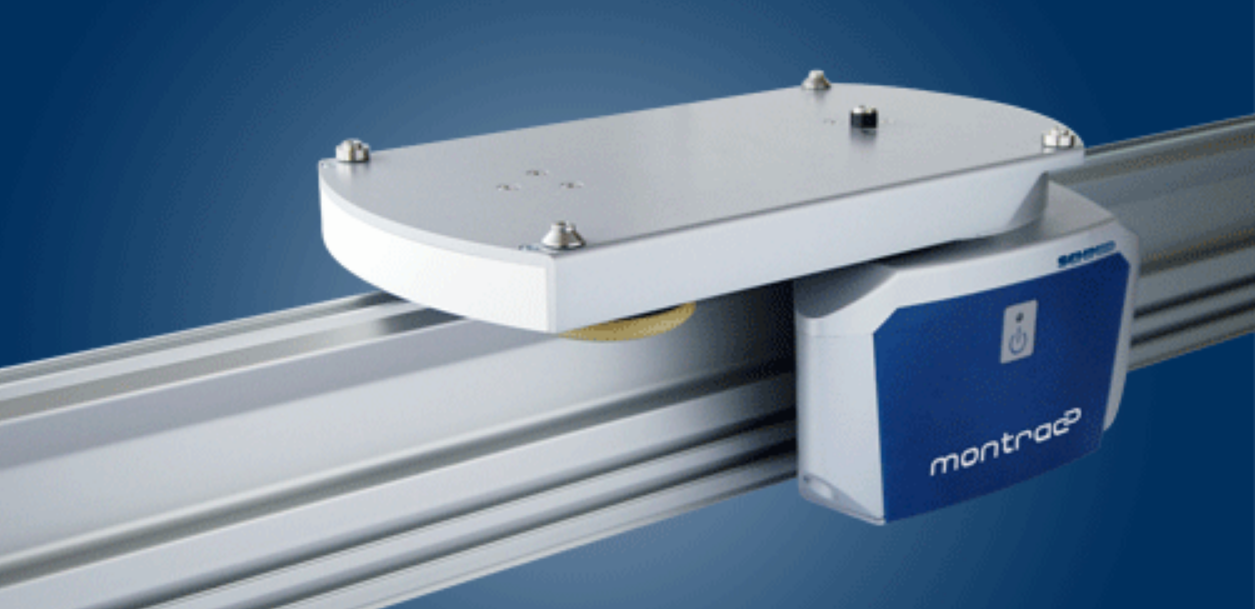
\includegraphics[scale=0.4]{Images/page_garde.png}
\end{center} 
\end{figure} 

\vspace{1cm}

{\LARGE Auteurs}\\

\vspace{0.5cm}

Bruno \bsc{Dato}, Abdellah \bsc{Elgourain} et Evgeny \bsc{Shulga}\\

\vspace{1cm}

{\Large Encadrants}\\

\vspace{0.5cm}

C. Briand, E. Le Corronc, L. Houssin \\ 

\vspace{3cm}


27 mai 2016




\end{center}

\newpage
\addcontentsline{toc}{section}{Remerciements}
\chapter*{Remerciements}

Nous tenons à remercier nos encadrants de projet E. Le Corronc, L. Houssin et C. Briand pour nous avoir guidés tout au long de ce projet et avoir répondu à nos questions. Nous les remercions également pour les conseils qu'ils nous ont apportés durant la rédaction du rapport.\\

Nous remercions aussi toutes les personnes de l'AIP pour leur accueil au sein de la halle technologique, particulièrement T. Canzonieri qui nous a beaucoup aidé pour la prise en main de tous les outils que nous avons utilisés durant notre projet.

\newpage
\renewcommand{\contentsname}{Sommaire} % permet de changer le titre de la table des matières
\tableofcontents %sommaire


\newpage
\addcontentsline{toc}{section}{Introduction}
\chapter*{Introduction}


Afin d'enrichir et développer nos capacités de recherche scientifique, notre formation Master EEA, option Ingénierie des Systèmes Temps Réel, nous permet d'effectuer un projet d'initialisation à la recherche. Ce projet est un travail de groupe qui démarre pendant le premier semestre et qui se termine par une présentation orale à la fin du second semestre.\\

Le sujet que nous avons choisi est la commande d'une ligne transitique MONTRAC via ROS (Robot Operating System), qui est un outil informatique très utilisé pour développer des applications dans le domaine de la robotique. La ligne transitique se trouve à la Halle technologique sur le campus de l'université Paul Sabatier.\\

Nous avons tout d'abord commencé par une phase de recherche bibliographique pendant laquelle nous nous sommes documenté sur les travaux déjà effectué sur la ligne transitique et en parallèle nous nous sommes formés au langage C++ qui était nouveau pour certaines personnes du groupe et qui serait utile pour la prise en main de ROS. Nous sommes ensuite passés au sujet principal de notre projet, commander la ligne transitique et sa simulation qui a été conçue par un groupe d'étudiants cette même année.\\


Nous commencerons dans une premier temps par présenter le projet ainsi que sont environnement. Dans cette partie, nous détaillerons le fonctionnement de la ligne transitique et de la simulation. Ensuite, nous présenterons la solution envisagée pour la commande via ROS. Nous terminerons par présenter le fonctionnement de ROS.\\

Dans un second temps, nous expliquerons quels sont les configurations de la ligne transitique plus particulièrement de ses automates requises afin de pouvoir implémenter une commande. Nous détaillerons dans cette partie comment nous avons établi la communication avec la ligne.\\

Enfin, dans la dernière partie de ce projet, nous décrirons le fonctionnement de la commande et nous présenterons deux exemples de commandes que nous avons réalisées.\\

\newpage
\begin{figure}[H]
	     \begin{center}
	     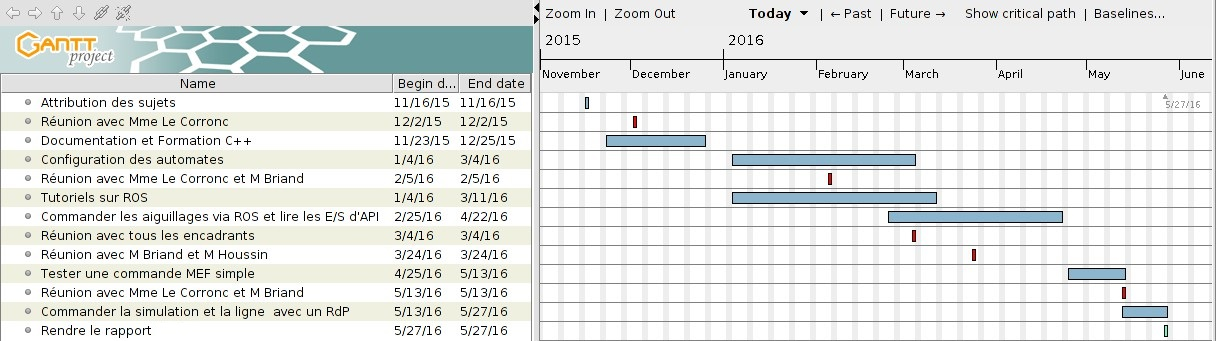
\includegraphics[angle=90,scale=0.8]{Images/Gantt.jpg} 
	     \end{center}
	     \caption{Diagramme de GANTT}
	     \label{Gantt}
\end{figure}


\newpage
\chapter{Présentation du projet}

\section{Pôle AIP/PRIMECA Toulouse}

\vspace{0.2cm}

\begin{wrapfigure}[12]{r}{6.8cm}
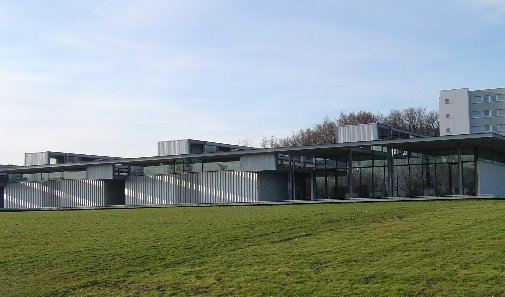
\includegraphics[scale=0.4]{Images/halle.jpg}
\caption{Halle technologique Paul Sabatier}
\label{Halle technologique Paul Sabatier}
\end{wrapfigure}

L'Université Paul Sabatier, l'INP Toulouse, l'INSA Toulouse et le LAAS-CNRS ont développé dès 1983 une politique de site afin de renforcer la formation pratique dans certains domaines nécessitants des moyens lourds et couteux, en phase avec la réalité industrielle. Cette politique de mutualisation des ressources et des compétences s'est traduite par la création de trois ateliers inter-universitaires : l'AIGEP dans le domaine du Génie des Procédés, l'AIME dans le domaine de la Micro-nano-électronique, et l'AIP-PRIMECA dans les domaines de la Mécanique et de la Productique. Le pôle AIP-PRIMECA toulousain fait partie d'un réseau national composé de 9 pôles régionaux.\\

\vspace{0.8cm}

Le pôle AIP-PRIMECA Toulouse est implanté sur deux sites :
\begin{itemize}
\item[ ]
\item[•] l'Université Paul Sabatier (halle technologique)
\item[•] l'INSA Toulouse (Département Génie Mécanique)
\item[ ]
\end{itemize}

L'AIP-PRIMECA, ou l'Atelier Inter-établissements de Productique et Pôle de Ressources Informatiques pour la MECAnique, est un réseau, comptant 9 antennes réparties sur le territoire français, qui contribue au regroupement d'établissements d'enseignement supérieur dont l'objectif est d'offrir les ressources humaines et les moyens matériels afin de développer des projets universitaires et de valoriser la formation des étudiants dans le domaine de l'industrie. Cet établissement soutien aussi des activités de recherche.\\

Ce local situé dans la halle technologique comporte des salles de cours et de TP équipées de différents systèmes tels que des robots mobiles, des robots manipulateurs ainsi que la ligne transitique MONTRAC$^{\circledR}$ à laquelle s'intéresse notre projet et qui dans un avenir proche sera destinée à accueillir des TP et des projets.\\ 

\newpage
\section{Ligne transitique MONTRAC$^{\circledR}$}

\subsection{Présentation}

La ligne transitique MONTRAC est composée de rails alimentés en énergie électrique sur lesquels circulent des navettes. Les navettes ne peuvent se déplacer que dans un sens sur ces rails.\\
     
Pour commander la ligne, on dispose de cinq automates programmables industriels que nous appellerons API. Il y en a 2 de la marque Siemens$^{\circledR}$ et 3 de type Schneider$^{\circledR}$. Ces automates gèrent les différents actionneurs et capteurs situés sur les rails. Les navettes ne sont pas programmables, une fois allumées elles avancent jusqu'à ce qu'on les arrête. Elles possèdent un capteur de proximité situé à l'avant pour éviter les collisions entre les navettes et les stopper lorsqu'elles rencontrent un obstacle.\\       

Cette ligne comporte 5 "secteurs" dont un central et 4 postes de travail. Chaque "secteur" est contrôlé par un des API qui agit sur la ligne via un système d'air comprimé. Les zones 1 à 3 correspondent aux automates Schneider$^{\circledR}$ et les deux autres zones correspondent aux automates Siemens$^{\circledR}$. La ligne possède 12 aiguillages comme on peut le voir sur la figure \ref{Les zones de travail}.

\begin{figure}[H] 
\begin{center}
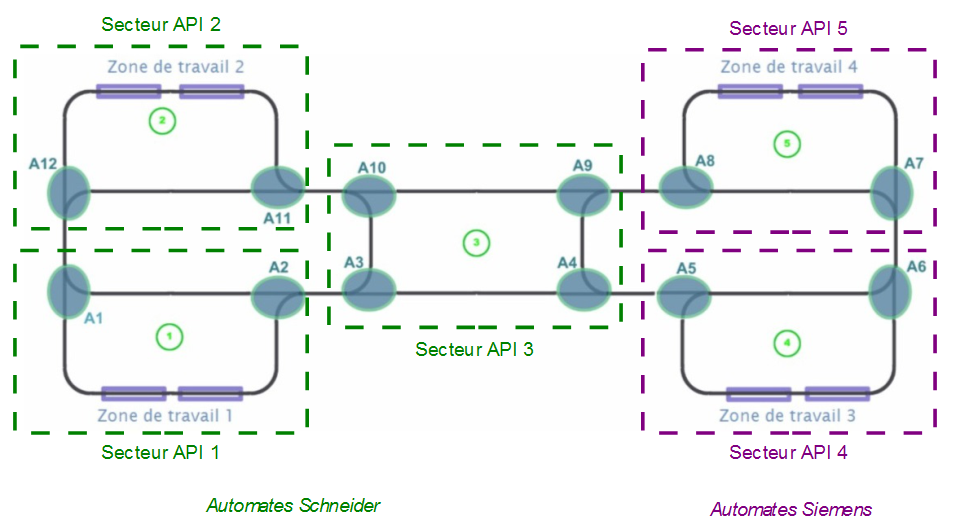
\includegraphics[scale=0.65]{Images/zone_travail.png} 
\end{center}
\caption{Schéma simplifié de la ligne transitique}
\label{Les zones de travail}
\end{figure} 

Chaque automate n'ayant accès qu'à une partie de la cellule, il est nécessaire de les faire communiquer entre eux afin de commander les navettes sur l'ensemble de la ligne.\\

\newpage
\subsection{Capteurs et actionneurs}

Les actionneurs permettent de commander les points d'arrêts des navettes, les aiguillages et des ergots pouvant bloquer les navettes à certains endroits lorsqu'elles sont arrêtées. Les capteurs nous permettent de connaître les positions des navettes, des aiguillages et des ergots. Les listes des actionneurs et capteurs sont données ci-dessous.

\begin{table}[H]

 
\begin{center}
\begin{tabular}{|c||l|}
	\hline RxG   & Positionne l'aiguillage x à gauche  \\
	\hline RxD   & Positionne l'aiguillage x à droite  \\
	\hline Dx    & Dévérrouille l'aiguillage X          \\
	\hline Vx    & vérrouille l'aiguillage X            \\
	\hline STx   & Quand STx vaut 0, les navettes s'arrêtent au niveau de l'actionneur \\
	\hline PIx    & Blocage des navettes sur le poste de travail \\
	\hline
\end{tabular}     
\end{center}
\caption{\label{tab:actionneurs}Actionneurs}
\end{table}
\

\begin{table}[H]

 	  
\begin{center}
	\begin{tabular}{|c||l|}
	\hline CPx   & Capteur de Position. Vaut 1 quand une navette est sur le capteur \\
	\hline PSx   & Capteur de Stop situé juste en face d'un actionneur STx pouvant arrêter la navette \\
	\hline CPIx  & Vaut 1 quand l'ergot PI est sorti      \\
	\hline DxD   & Vaut 1 quand l'aiguillage x est à droite         \\
	\hline DxG   & Vaut 1 quand l'aiguillage x est à gauche \\
	\hline
	\end{tabular}        
\end{center}
\caption{\label{tab:capteurs}Capteurs}
\end{table}

Durant ce projet, nous nous sommes concentrés sur la commande de la ligne via les API des zones 1 et 2 (automates Schneider$^{\circledR}$) car le rack réseau du 3\textsuperscript{ème} automate Schneider$^{\circledR}$ était endommagé et nous n'avons pas réussi à communiquer par réseau avec les automates Siemens$^{\circledR}$. La configuration des autres API est disponible dans le rapport de projet de l'année 2015 \hyperref[biblio]{\textbf{[1]}}.\\

Les automates 1 et 2 disposent de 16 entrées et sorties chacun mais toutes ne sont pas utilisées. Les tables \ref{tab:ap1} et \ref{tab:ap2} décrivent respectivement le câblage des API 1 et 2. \\

On peut voir sur la figure~\ref{Schema_detaille} une vision globale de la ligne transitique avec tous les capteurs et actionneurs, les zones contrôlées par les API ainsi que les orientations de chaque rail.

\newpage
\begin{center}
\Rotatebox{90}{%
\begin{minipage}{1.5\linewidth}
\begin{table}[H]
	\begin{center}
		\begin{tabular}{|c|c|c|c|c|c|c|c|c|c|c|c|c|c|c|c|c|c|c|c|c|c|c|c|}
			\hline \multicolumn{2}{|c|}{\textbf{OUT}}  & \multicolumn{2}{|c|}{A1} & \multicolumn{2}{|c|}{V1} & \multicolumn{2}{|c|}{A2} & \multicolumn{2}{|c|}{V2} & \multicolumn{2}{|c|}{S1} & \multicolumn{2}{|c|}{S2} & \multicolumn{2}{|c|}{S3} & \multicolumn{2}{|c|}{S4} & \multicolumn{2}{|c|}{S5} & \multicolumn{2}{|c|}{UP1} & \multicolumn{2}{|c|}{UP2}  \\
			\hline \multicolumn{2}{|c|}{} & R1D & R1G & V1 & D1 & R2D & R2G & V2 & D2 & \multicolumn{2}{|c|}{ST1} & \multicolumn{2}{|c|}{ST2} & \multicolumn{2}{|c|}{ST3} & \multicolumn{2}{|c|}{ST5} & \multicolumn{2}{|c|}{ST4} & \multicolumn{2}{|c|}{PI1} & \multicolumn{2}{|c|}{PI2} \\
			\hline \multicolumn{2}{|c|}{\textbf{IN}} & 0 & 1 & 2 & 3 & 4 & 5 & 6 & 7 & 8 & 9 & 10 & 11 & 12 & 13 & 14 & 15 & & & & & & \\
			\hline \multicolumn{2}{|c|}{} & PS1 & PS2 & PS3 & PS5 & PS4 & D1D & D1G & CP1 & CPI1 & CPI2 & D2D & D2G & CP2 & PS6 & & & & & & & & \\
			\hline
		\end{tabular}     
	\end{center}
	\caption{\label{tab:ap1}Configuration des entrées/sorties de l'automate Schneider 1}

\end{table}

\begin{table}[H]
	\begin{center}
		\begin{tabular}{|c|c|c|c|c|c|c|c|c|c|c|c|c|c|c|c|c|c|c|c|c|c|c|c|}
			\hline \multicolumn{2}{|c|}{\textbf{OUT}}  & \multicolumn{2}{|c|}{A1} & \multicolumn{2}{|c|}{V1} & \multicolumn{2}{|c|}{A2} & \multicolumn{2}{|c|}{V2} & \multicolumn{2}{|c|}{S1} & \multicolumn{2}{|c|}{S2} & \multicolumn{2}{|c|}{S3} & \multicolumn{2}{|c|}{S4} & \multicolumn{2}{|c|}{S5} & \multicolumn{2}{|c|}{UP1} & \multicolumn{2}{|c|}{UP2}  \\
			\hline \multicolumn{2}{|c|}{} & R11D & R11G & V11 & D11 & R12D & R12G & V12 & D12 & \multicolumn{2}{|c|}{ST20} & \multicolumn{2}{|c|}{ST21} & \multicolumn{2}{|c|}{ST22} & \multicolumn{2}{|c|}{ST24} & \multicolumn{2}{|c|}{ST23} & \multicolumn{2}{|c|}{PI7} & \multicolumn{2}{|c|}{PI8} \\
			\hline \multicolumn{2}{|c|}{\textbf{IN}} & 0 & 1 & 2 & 3 & 4 & 5 & 6 & 7 & 8 & 9 & 10 & 11 & 12 & 13 & 14 & 15 & & & & & & \\
			\hline \multicolumn{2}{|c|}{} & PS20 & PS21 & PS22 & PS24 & PS23 & D11D & D11G & CP9 & CPI7 & CPI8 & D12G & D12G & CP10 & PS1 & & & & & & & & \\
			\hline
		\end{tabular}      
	\end{center}
	\caption{\label{tab:ap2}Configuration des entrées/sorties de l'automate Schneider 2}
\end{table}
\end{minipage}
}%
\end{center}



\begin{figure}[H]
	     \begin{center}
	     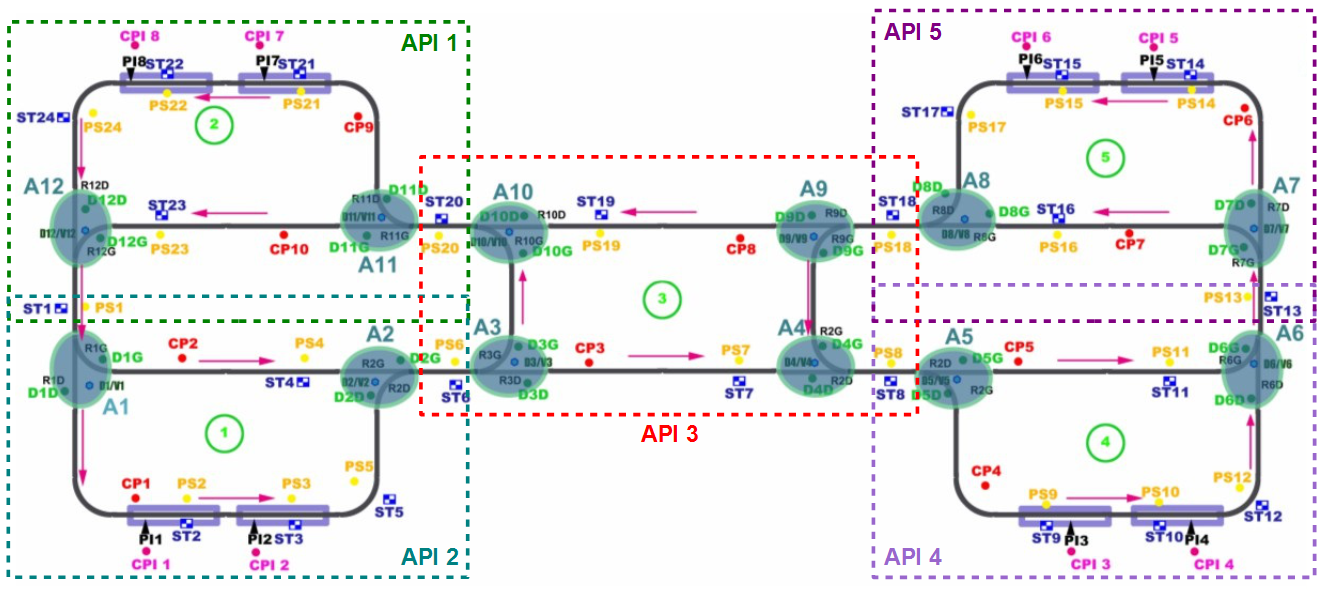
\includegraphics[angle=90,scale=0.72]{Images/maquette.png} 
	     \end{center}
	     \caption{Schéma détaillé de la ligne transitique}
	     \label{Schema_detaille}
\end{figure}

\section{Simulation de la ligne transitique} 

En parallèle de notre projet, un groupe d'étudiants de l'ENSEEIHT a conçu une simulation de la ligne transitique à l'aide du logiciel V-REP\footnote{V-REP est une plateforme de simulation pour tout type de robots \hyperref[biblio]{\textbf{[7]}}.}. Cette simulation se comporte comme la ligne MONTRAC$^{\circledR}$, bien qu'elle ne possède pas tous les capteurs et actionneurs (nous détaillerons les différences table \ref{tab:capteur_simu}). Elle permet de valider un grand nombre de commandes avant des les tester directement sur la ligne réelle. Le but final serait de créer un TP dans lequel les étudiants testeraient tout d'abord leur commande sur la simulation et une fois celle-ci validée, ils pourraient la tester sur le système réel.

\begin{figure}[H]
	     \begin{center}
	     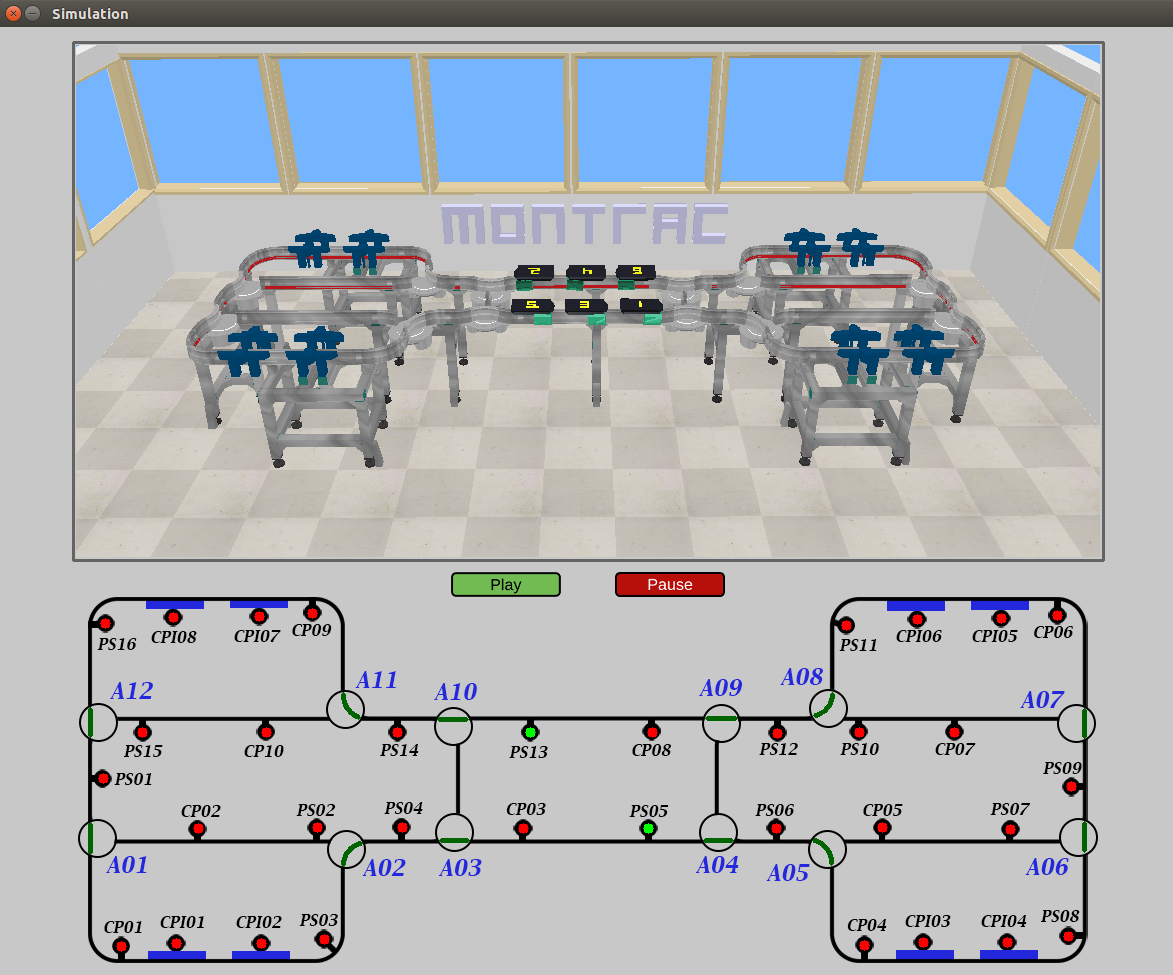
\includegraphics[scale=0.5]{Images/simulation2.png} 
	     \end{center}
	     \caption{Simulation de la ligne transitique}
	     \label{Simulation}
\end{figure}

Pour la conception de la simulation, les étudiants on regroupé les capteurs en catégories : CPI, CP, PS, DG et DD qui correspondent à ceux cités précédemment (table~\ref{tab:capteurs}). Il y a cependant quelques différences pour les capteur PS et CPI comme on peut le voir sur la table \ref{tab:capteur_simu}.


\begin{table}[H]

 	  
\begin{center}
	\begin{tabular}{|c||c|c|c|c|c|c|c|c|c|c|c|c|c|}
	\hline Ligne transitique   &PS1&PS2&PS3&PS4&PS5&PS6&PS7&PS8&PS9&PS10&PS11&PS12&PS13\\
	\hline Simulation   &PS1&CPI1&CPI2&PS2&PS3&PS4&PS5&PS6&CPI3&CPI4&PS7&PS8&PS9\\
	\hline
	\end{tabular} 
	\\[0.7cm]
	\begin{tabular}{|c||c|c|c|c|c|c|c|c|c|c|c|}
	\hline Ligne transitique   &PS14&PS15&PS16&PS17&PS18&PS19&PS20&PS21&PS22&PS23&PS24\\
	\hline Simulation   &CPI5&CPI6&PS10&PS11&PS12&PS13&PS14&CPI7&CPI8&PS15&PS16\\
	\hline
	\end{tabular}       
\end{center}
\caption{\label{tab:capteur_simu}Capteurs de stop de la ligne transitique et de la simulation}
\end{table}

\newpage
Sur la simulation, les capteur CPI ne sont pas les capteurs de position des ergots mais des capteurs de stop aussi. Pour les actionneurs, il y a 5 registres : RD, RG, LOCK, STOP et GO ; RD et RG fonctionnement de la même manière que ceux de la table~\ref{tab:actionneurs} mais LOCK, STOP et GO ont un fonctionnement différent :

\begin{itemize}
\item[ ]
\item[•] LOCKx = $\overline{\text{Vx}}$.Dx
\item[•] STOPx = $\overline{\text{STx}}$
\item[•] GOx = STx
\item[ ]
\end{itemize}




\section{Problématique et solution mise en place}

Comme nous l'avons dit précédemment, chaque API commande une seule partie de la ligne transitique et n'a pas accès au reste de la ligne. Afin de commander la ligne dans sa globalité, il est nécessaire de faire communiquer l'ensemble des automates en réseau. Pour cela, afin de remplir l'objectif principal de ce TER, nous avons utilisé le logiciel de libre accès ROS (Robot Operating System), c'est un ensemble de librairies et d'outils qui permettent de mettre en place toutes sortes d'applications robotiques. Concrètement, il permet d'établir des ponts de communication entre divers systèmes.\\

Le deuxième objectif était de pouvoir commander la simulation de la même façon que la ligne transitique afin de pouvoir valider différents scénarios avant les tests réels. La simulation fonctionnant également à l'aide de ROS,
nous avons pu mettre en place une même commande que ce soit pour la simulation ou la ligne transitique.\\

Enfin, chaque commande implémentée sur notre système a été modélisée par des machines à état finis (MEF) au début pour des commandes simples. Puis par la suite, ces commandes ont été modélisées par des réseaux de Petri (RdP) pour les commandes nécessitant du parallélisme et comportant plusieurs navettes.\\

Pour répondre à tous ces objectifs, nous avons donc réalisé un pont de communication à l'aide de ROS entre la commande modélisée par une MEF ou un RdP et la simulation/ligne transitique (figure \ref{schema_solution}).

\begin{figure}[H] 
\begin{center}
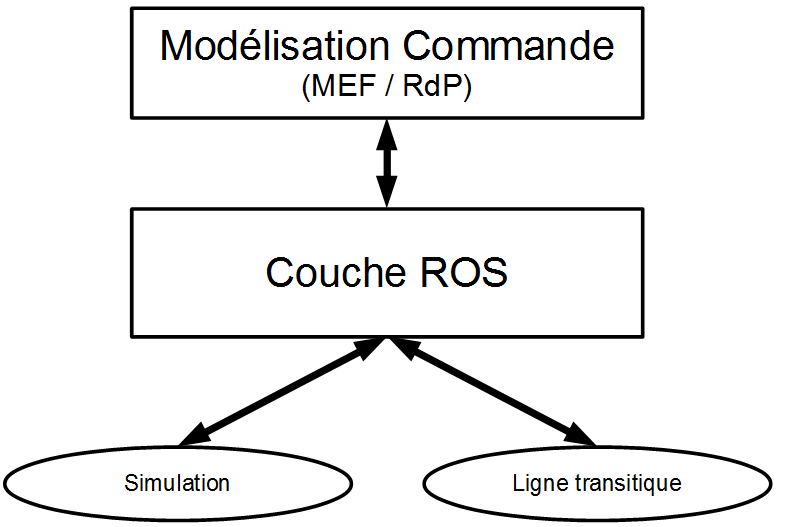
\includegraphics[scale=0.4]{Images/solution.png} 
\end{center}
\caption{Architecture de la solution mise en place}
\label{schema_solution}
\end{figure} 



\section{Présentation de ROS\label{section_pre_ros}}

ROS (Robot Operating System) est une plateforme de développement logiciel qui facilite le développement d'applications robotiques car il permet de créer des pont de communication entre différentes entités de façon très simple. ROS peut être implémenté dans 2 langages : le Python et le C++, nous avons choisi le C++.\\

ROS permet l'échange de messages entre nœuds qui sont stockés dans des répertoires nommés packages. Les nœuds sont des exécutables qui utilisent ROS afin de communiquer avec d'autres nœuds. Pour que les nœuds puissent communiquer entre eux, il faut lancer la plateforme en activant un maître (annexe \ref{annexe_ROS_compilation}). Les nœuds peuvent échanger alors les informations entre eux soit de manière asynchrone via un topic (sujet) ou de manière synchrone via un service\footnote{Pour notre projet nous n'avons pas utilisé de services.}. Chaque nœud ROS évolue en parallèle par rapport aux autres.\\

Le principe des topics est assez simple, il est possible de publier sur un topic ou bien d'y être abonné. Lorsqu'un nœud publie sur un topic, il envoie un message à des instants choisis par le programmeur (à une certaine fréquence ou sous certaines conditions). Lorsqu'un nœud est abonné à un topic, il reçoit tous les messages publiés sur ce topic et pour chaque message reçu, une fonction appelée "Callback" est lancée afin de traiter le message comme on le souhaite. Il est possible de publier sur plusieurs topics et d'être abonné à plusieurs topics à la fois. Pour publier et lire des messages sur un topic, il faut aussi définir les types de messages que l'on souhaite utiliser.


\begin{figure}[H] 
\begin{center}
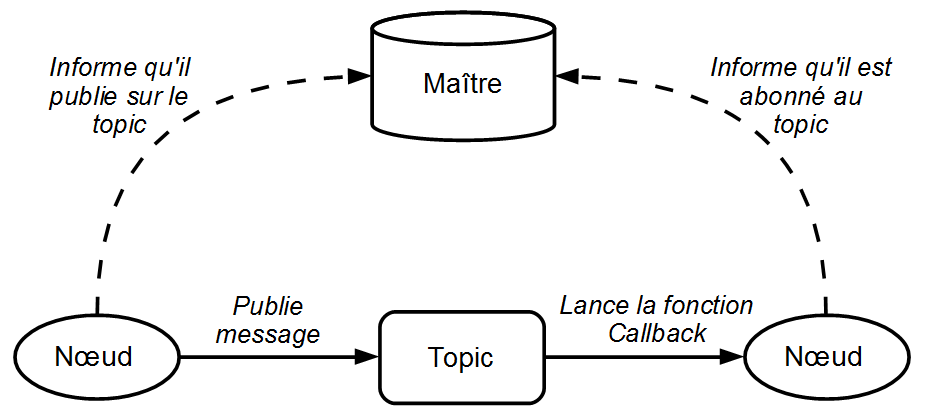
\includegraphics[scale=0.4]{Images/topic.png} 
\end{center}
\caption{Fonctionnement d'un topic sur ROS}
\label{topic}
\end{figure} 


\newpage

\chapter{Communication avec les automates}

Avant de commander la ligne transitique, nous avons tout d'abord dû établir la communication avec les automates en configurant premièrement les API 1 et 2 à l'aide du logiciel PL7-PRO. Nous avons ensuite ajouté une couche ROS de communication pure permettant d'obtenir les valeurs des toutes les entrées et sorties des automates considérés pour les envoyer ensuite à la couche ROS de commande que nous détaillerons par la suite. La communication entre les automates et ROS se fait par un protocole Modbus TCP/IP que nous détaillerons.

\vspace{2cm}

\begin{figure}[H] 
\begin{center}
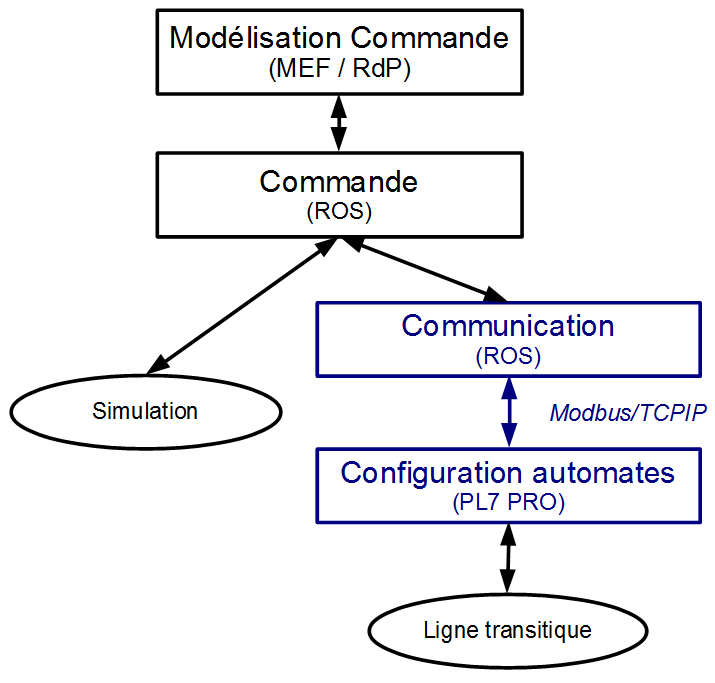
\includegraphics[scale=0.5]{Images/communication.png} 
\end{center}
\caption{Architecture de la solution mise en place avec la couche de communication}
\label{com}
\end{figure} 


\newpage
\section{Configuration des automates Schneider}

Dans cette partie nous allons décrire brièvement les différents étapes pour configurer les API Schneider$^{\circledR}$ via PL7-PRO. Puis nous validerons le bon fonctionnement des automates à l'aide de différents tests.
    
\subsection{Configuration matérielle et logicielle}

Tout d'abord, lorsque l'on crée un fichier de configuration pour un automate sur PL7-PRO, il faut choisir le processeur que l'on utilise, ici c'est le TSX 57103 V5.1. Ensuite, on définit les types de racks utilisés c'est à dire la configuration matérielle (figure~\ref{config_materielle}) de l'automate puis sa configuration logicielle (figure \ref{config_logicielle}). On fait un fichier pour chaque automate à utiliser pour commander la ligne transitique. Dans notre cas, nous ne configurons que 2 automates.


\begin{figure}[H] 
  \centering
  \subfloat[Configuration matérielle des API 1 et 2]{\label{config_materielle}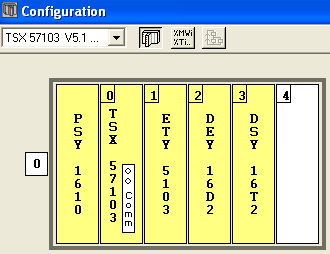
\includegraphics[scale=0.8]{Images/Configuration_materielle.png}}
  \hspace{20pt}
  \subfloat[Configuration logicielle des API 1 et 2]{\label{config_logicielle}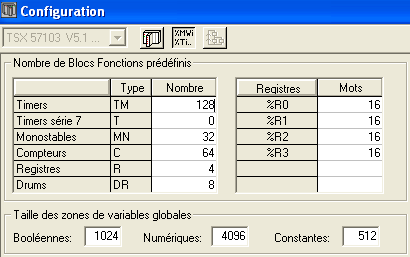
\includegraphics[scale=0.8]{Images/Configuration_logicielle.png}}  
  \caption{Configuration des API 1 et 2}
  \label{config_ap12}
\end{figure}

On choisi en cliquant sur les racks figure \ref{config_materielle} les paramètres et modules suivants : 

\begin{itemize}
\item[ ] 
\item[ ] TSX RKY 6 : le nombre de racks(6 POSITIONS NON EXTENSIBLE\footnote{Cliquez sur le 0 dans le carré blanc pour modifier ce paramètre})
\item[ ] TSX PSY 1610 : l'alimentation de l'API (ALIM. 24VCC NON ISOL. 16W),
\item[0.] TSX 57103 : le processeur (il possible de le choisir ici aussi, ne pas modifier les paramètres par défaut),
\item[1.] TSX ETY 5103 : le module réseau que l'on détaillera plus tard,
\item[2.] TSX DEY 16D2 : les entrées (capteurs) de l'API,
\item[3.] TSX DSY 16T2 : les sorties (actionneurs) de l'API.
\item[ ]
\end{itemize}


\subsection{Mise en réseau des automates\label{section_reseau}}

Afin de communiquer avec les automates en utilisant le réseau local de l'AIP, on configure les modules réseau de chacun des 2 automates avec les adresses suivantes (exemple de configuration figure \ref{config_reseau_ap1}) :

\begin{center}
\begin{tabular}{cc}
Adresse IP API 1 & 192.168.0.101\\
Adresse IP API 2 & 192.168.0.102\\
Masque sous-réseau & 255.255.255.0\\
Adresse du Gateway & 192.168.0.13\\
\end{tabular}
\end{center}


\begin{figure}[H] 
\begin{center}
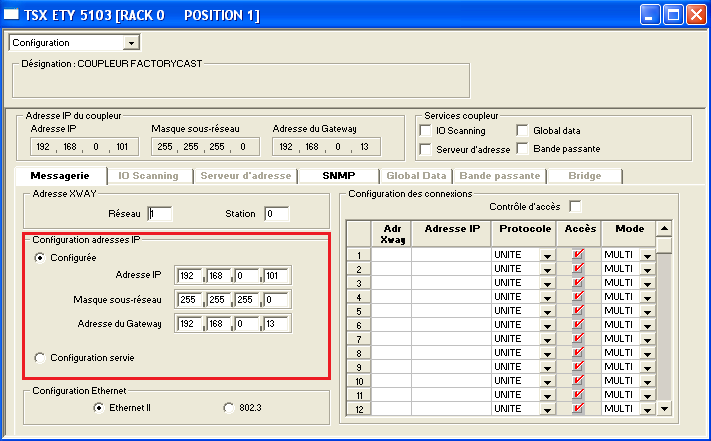
\includegraphics[scale=0.8]{Images/reseau.png} 
\end{center}
\caption{Configuration réseau de l'API 1}
\label{config_reseau_ap1}
\end{figure} 

Une fois ces configurations faites, il faut veiller à brasser les deux automates. C'est à dire qu'il faut brancher les câbles réseau qui partent des automates sur un switch pour qu'ils soient connectés au réseau. Dans ce cas, le swtich est situé dans une armoire de brassage.


\subsection{Mémoire partagée}

Maintenant qu'il est possible d'échanger des informations via le réseau, on déclare des variables au sein des 2 automates pour chaque capteur et actionneur. Ces variables sont définies dans Variables/Objets Mémoire dans le navigateur (figure \ref{navigateur}). Nous avons utilisé deux mots de 16 bits (type WORD) pour chaque API (figure \ref{memoire_ap1}). Le mot MW0 pour les sorties/actionneurs et le mot MW1 pour les entrées/capteurs. Chaque bit correspond alors à un actionneur pour MW0 ou à un capteur pour MW1 avec la même numérotation que dans les tables \ref{tab:ap1} et \ref{tab:ap2}.

On assigne ensuite aux variables correspondant aux capteurs MW1:X[0..13] les valeurs des entrées de l'automate I2[0..13] et on assigne aux sorties de l'automate Q3[0..14] les valeurs des variables correspondant au actionneurs MW0:X[0..14] (programme figure \ref{prog_ap1}). Ainsi, on peut connaître l'état d'un capteur en lisant le mot MW1 et on peut définir les sorties à actionner en écrivant dans le mot MW0.

Le programme de l'API 2 est exactement le même, seulement le nom des capteurs et actionneurs change pour les Objets mémoire. La mémoire ainsi créée sera partagée par les automates et par la couche ROS qui pourra lire et écrire dans cette mémoire.


\begin{figure}[H] 
  \centering
  \subfloat[Navigateur d'application]{\label{navigateur}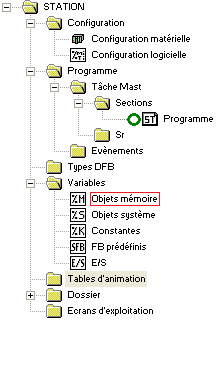
\includegraphics[scale=0.85]{Images/navigateur.png}}
  \hspace{20pt}
  \subfloat[Objets mémoire API 1]{\label{memoire_ap1}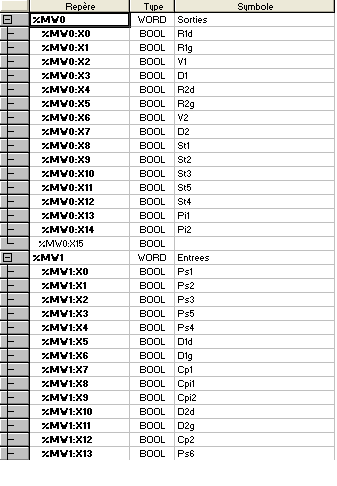
\includegraphics[scale=0.75]{Images/memoire.png}}  
  \hspace{20pt}
  \subfloat[Programme API 1]{\label{prog_ap1}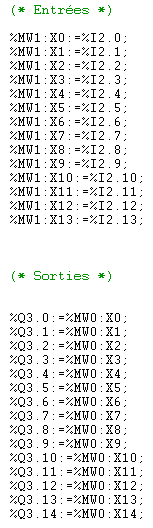
\includegraphics[scale=0.7]{Images/prog.png}}  
  \caption{Mise en place des variables partagés pour l'API 1}
  \label{config_ap12}
\end{figure}

\subsection{Validation}

\subsubsection{Connexion au réseau}

Afin de vérifier que les automates étaient bien connectés au réseau, nous avons utilisé la commande \textbf{ping} qui suivie de l'adresse IP de l'appareil que l'on souhaite tester nous permet de savoir s'il est connecté au réseau. Cette commande fournit aussi le temps écoulé entre la requête envoyée par la commande \textbf{ping} et la réponse donnée par l'appareil.

\begin{figure}[H] 
\begin{center}
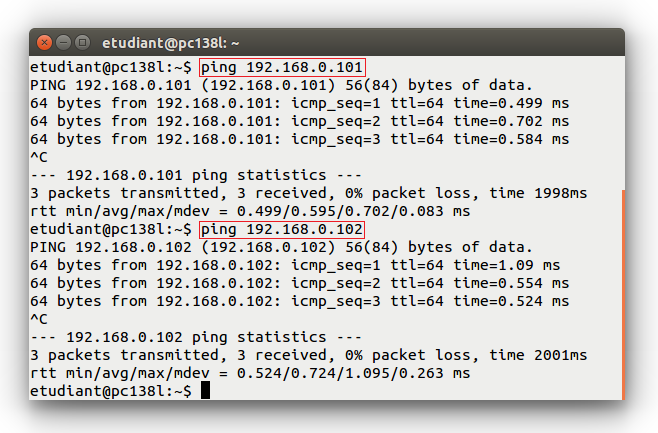
\includegraphics[scale=0.7]{Images/ping.png} 
\end{center}
\caption{Test de mise en réseau des API 1 et 2}
\label{ping}
\end{figure}

On peut voir sur la figure \ref{ping} que les automates 1 et 2 répondent aux requêtes envoyés par le \textbf{ping} ce qui prouve qu'ils sont bien connectés au réseau.

\subsubsection{Test de la mémoire partagée}

Pour tester le bon fonctionnement de la mémoire partagée mais aussi de la ligne transitique, après avoir lancé le mode RUN sur les 2 API configurés, nous avons observé la table animée sur PL7-PRO figure  \ref{animee}. On observe alors que lorsqu'une entrée de l'API prend la valeur 1, la variable partagée associé prend cette même valeur (cadre vert). Et lorsque l'on met à 1 une variable associée à une sortie de l'API, celle ci s'active (cadres rouges). Il est aussi possible de forcer directement les sorties et entrées de l'automate et observer les variables partagées évoluer de la même manière.

Nous avons pu de même nous familiariser avec le fonctionnement général de la ligne en testant les différents actionneurs notamment en utilisant les aiguillages qui nécessitent d'être déverrouillés avant chaque déplacement puis verrouillés une fois le déplacement terminé.

\begin{figure}[H] 
\begin{center}
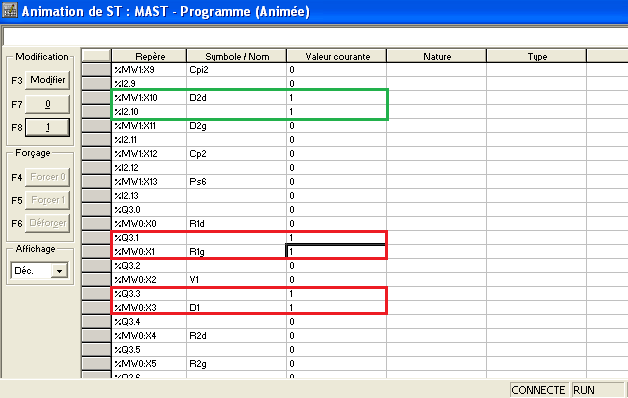
\includegraphics[scale=0.8]{Images/animee.png} 
\end{center}
\caption{Partie de la table animée de API 1}
\label{animee}
\end{figure}

\newpage
\section{Couche ROS de communication}

Afin de créer le pont de communication sous ROS que nous avons présenté précédemment nous avons utilisé 3 nœuds ROS : les noeuds \emph{Automates} et \emph{Communication} que nous allons présenter dans ce chapitre et le nœud \emph{Commande} que nous détaillerons plus tard. Ces 3 noeuds échangent des données à l'aide des topics \emph{Entrées API} 1 et 2, \emph{Sorties API} 1 et 2, \emph{Capteurs} et \emph{Actionneurs}. Pour échanger ces données, nous avons définit 4 types de messages différents : \emph{Entrées}, \emph{Sorties}, \emph{Actionneurs} et \emph{Capteurs}. Les messages \emph{Entrées} et \emph{Sorties} correspondent exactement aux entrées et sorties de chaque API. Les messages \emph{Actionneurs} et \emph{Capteurs} regroupent respectivement toutes les entrées des API en un mot de données et toutes les sorties des API en un seul autre mot.\\

Le nœud \emph{Automates} permet de lire les entrées de chaque automates par liaison Modbus TCP/IP et les envoyer au nœud \emph{Communication} mais aussi de recevoir les sorties données par le nœud \emph{Communication} et de les écrire dans les automates toujours par liaison Modbus TCP/IP. Le nœud \emph{Communication} concatène les messages \emph{Entrées API} des différents automates en un seul message \emph{Capteurs} à destination de la commande et il décompose le message \emph{Actionneurs} reçu en plusieurs messages \emph{Sorties API} à destination des différents automates.\\

La figure \ref{schema_detail} représente l'ensemble des nœuds, topics et messages ainsi que leur organisation générale.\\

\vspace{1.5cm}

\begin{figure}[H] 
\begin{center}
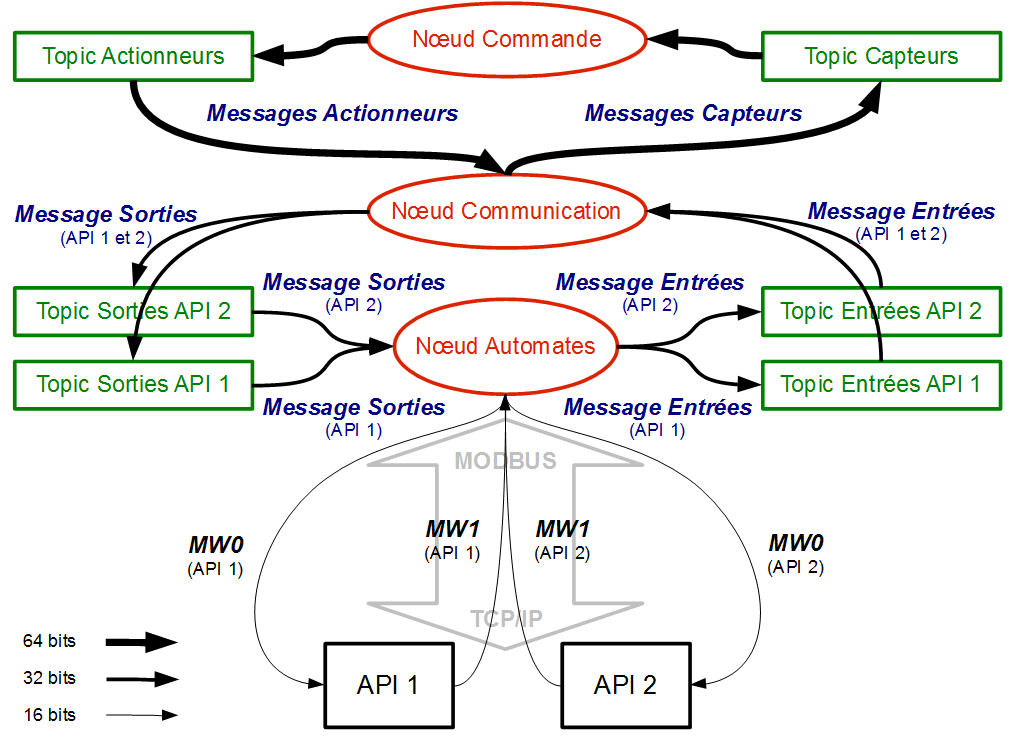
\includegraphics[scale=0.6]{Images/communication_ROS.png} 
\end{center}
\caption{Architecture détaillée de la communication via ROS entre le noeud de commande et les API}
\label{schema_detail}
\end{figure}

\newpage
\subsection{Liaison Modbus TCP/IP\label{section_modbus}}

\begin{wrapfigure}[16]{r}{5cm}
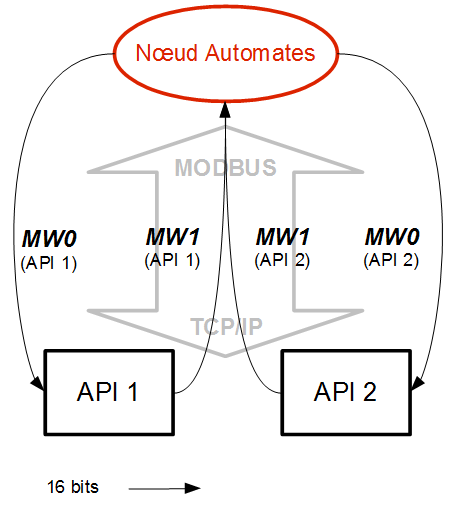
\includegraphics[scale=0.4]{Images/noeud_automates_modbus.png}
\caption{Échange de données entre le nœud \emph{Automates} et les API par liaison Modbus TCP/IP}
\label{modbus}
\end{wrapfigure}

Afin de mettre en œuvre la communication à l'échelle la plus basse avec les automates (figure \ref{modbus}), nous avons utilisé le protocole Modbus TCP/IP\footnote{Voir annexe \ref{annexe_modbus} pour l'installation des librairies.}.\\ 

Modbus TCP/IP (ou Modbus TCP) est un protocole de communication avec une interface TCP c'est à dire qui fonctionne sur Ethernet. Il fonctionne sur le mode Client/Serveur. Les clients sont tous actifs, le serveur est complètement passif. Chaque client lit et écrit dans le serveur. Chaque trame contient la fonction à traiter (écriture, lecture) et la donnée. L'adresse du serveur concerné est son adresse IP. C'est un protocole très répandu de part sa simplicité, sont coût nul et le peut de matériel requis. De même, il est très utilisé pour gérer les entrées et sorties de systèmes.\\

\vspace{1cm}

Pour établir le transfert de données nous avons utilisé les fonctions suivantes :

\begin{itemize}
\item[ ]
\item[•] \textbf{modbus\_new\_tcp(}\emph{adresse\_ip} , \emph{port\_logiciel}\textbf{)}\\
Elle permet d'initialiser la connexion avec un serveur à l'aide du paramètre \emph{adresse\_ip}. Pour le paramètre \emph{port\_logiciel}, on choisi le port par défaut (502). Cette fonction retourne un pointeur vers un élément de type \emph{modbus\_t} nécessaire à l'établissement de la connexion.
\item[ ]
\item[•] \textbf{modbus\_connect(}\emph{pointeur}\textbf{)}\\
Elle permet d'établir la connexion avec en paramètre le pointeur renvoyé par la fonction \textbf{modbus\_new\_tcp()}. Cette fonction retourne 0 si la connexion est établie et -1 sinon.
\item[ ]
\item[•] \textbf{modbus\_read\_registers(}\emph{pointeur , addresse\_registre , nombre\_registre , valeur\_sockée}\textbf{)}\\
Elle permet de lire un mot de 16 bit et de le stocker dans le paramètre \emph{valeur\_sockée}. Le paramètre \emph{pointeur} est toujours le même et \emph{adresse\_registre} correspond à l'adresse du registre qui est lu dans la mémoire des automates dans notre cas, c'est à dire les valeurs des entrées/capteurs (on a alors 1 comme adresse pour le mot \emph{MW1}). On ne lit qu'un seul registre à chaque fois donc le paramètre \emph{nombre\_registre} est toujours égal à 1. Cette fonction retourne le nombre de registres lus s'il n'y pas d'erreur et -1 sinon.
\item[ ]
\item[•] \textbf{modbus\_write\_register(}\emph{pointeur , addresse\_registre , valeur}\textbf{)}\\
Elle permet d'écrire un mot de 16 bits (\emph{valeur}) à l'\emph{addresse\_registre}. L'\emph{addresse\_registre} correspond dans notre cas à l'adresse de la mémoire correspondant au sorties/actionneurs des automates (0 pour \emph{MW0}). Cette fonction retourne 0 si l'écriture est réussie et -1 sinon.
\item[ ]
\item[•] \textbf{modbus\_close(}\emph{pointeur}\textbf{)} : Cette fonction ferme la connexion.
\item[ ]
\item[•] \textbf{modbus\_free(}\emph{pointeur}\textbf{)} : Cette fonction libère la mémoire utilisée pour le pointeur.
\end{itemize}



\subsection{Nœud ROS \textit{Automates}}

Mise à part les API avec lesquels le nœud \emph{Automates} communique par liaison Modbus TCP/IP, le nœud \emph{Automates} publie les messages \emph{Entrées} des API 1 et 2 respectivement sur les topics \emph{Entrées API 1} et \emph{Entrées API 2}. Il est aussi abonné au topics \emph{Sorties API 1} et \emph{Sorties API 2} qui lui envoient les messages \emph{Sorties} à destination des API 1 et 2 (figure \ref{schema_noeud_automates_topic}). Les messages \emph{Entrées} et \emph{Sorties} sont des types int32. La taille de ces messages est supérieure à celle des registres \emph{MW0} et \emph{MW1} lus sur les automates pour les cas où les entrées ou les sorties nécessitent 2 mots de 16 bits comme pour l'API 3 que nous n'avons pas pu utiliser.

\begin{figure}[H] 
\begin{center}
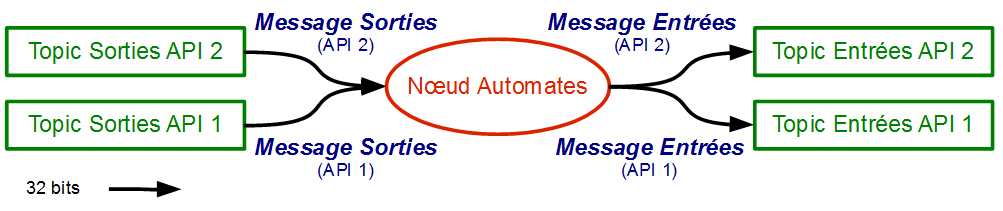
\includegraphics[scale=0.5]{Images/noeud_automates_topic.png} 
\end{center}
\caption{Nœud \emph{Automates} avec ses topics et messages}
\label{schema_noeud_automates_topic}
\end{figure}

\subsubsection{La classe API\_schneider}

Pour créer ce nœud, nous avons tout d'abord créé une classe API\_Schneider. Cette classe permet au nœud \emph{Automates} de publier sur les topics \emph{Entrées API} 1 et 2 et de s'abonner aux topics\emph{ Sorties API} 1 et 2.

\begin{center}
ATTRIBUTS
\end{center}

\begin{itemize}
\item[•] \textbf{pub\_entrées} : Objet de type Publisher disponible dans la librairie de ROS. Il permettra à la classe de publier sur un topic \emph{Entrées API}.
\item[•] \textbf{sub\_sorties} : Objet de type Subscriber disponible aussi dans la librairie de ROS. Il permettra à la classe de s'abonner à un topic \emph{Sorties API}.
\item[•] \textbf{adresse\_ip} : L'adresse IP de l'automate configurée dans la section \ref{section_reseau}.
\item[•] \textbf{entrées} : Les entrées de l'API.
\item[•] \textbf{sorties} : Les sorties de l'API.
\end{itemize}

\begin{center}
MÉTHODES
\end{center}

\begin{itemize}
\item[•] \textbf{API\_schneider(}\emph{noeud , num\_API , adresse\_ip\_api}\textbf{)}\\
C'est le constructeur de la classe, à l'aide des paramètre \emph{noeud} et \emph{num\_API} et il permet d'initialiser \textbf{pub\_entrées} et \textbf{sub\_sorties} en les reliant au nœud \emph{Automates} qui sera déclaré dans le main. On assigne \textbf{pub\_entrées} au topic \emph{Entrées API num\_API} et \textbf{sub\_sorties} au topic \emph{Sorties API num\_API}. Avec le paramètre \emph{adresse\_ip\_api}, on assigne à la classe l'adresse IP de l'automate correspondant. On initialise aussi les attributs \textbf{entrées} et \textbf{sorties}.
\item[ ]
\item[•] \textbf{get\_register(}\emph{adresse\_registre , nombre\_registres}\textbf{)}\\
Avec les paramètres \emph{adresse\_registr}e et \emph{nombre\_registres} décrits dans la section \ref{section_modbus}, cette fonction retourne le registre des entrées/capteurs de la mémoire partagée de l'automate considéré.
\item[ ]
\item[•] \textbf{write\_register(}\emph{adresse\_registre , nombre\_registres , registre}\textbf{)}\\
Avec les mêmes paramètres que la fonction précédente, cette méthode écrit le paramètre \emph{registre} sur la mémoire partagée correspondant aux sorties/actionneurs de l'automate considéré.
\item[ ]
\item[•] \textbf{Callback(}\emph{msg}\textbf{)}\\
Comme nous l'avons expliqué dans la section \ref{section_pre_ros}, cette fonction est appelée à chaque fois qu'un message de type \emph{Sorties} est publié sur le topic \emph{Sorties API num\_API} (paramètre \emph{msg}). Quand cela arrive, cette fonction actualise l'attribut \textbf{sorties} de la classe et envoie le message à l'automate avec la fonction \textbf{write\_register()}.
\item[ ]
\item[•] \textbf{publish()}\\
Cette méthode actualise l'attribut \textbf{entrées} de la classe à l'aide de la fonction \textbf{get\_register()} puis publie le message \emph{Entrées} sur le topic \emph{Entrées API num\_API}.
\end{itemize}


\subsubsection{Le main}

Dans le main (annexe \ref{annexe_automates_cpp}), on initialise et on déclare le nœud \textit{Automates}. Ensuite, on déclare deux objets de type API\_schneider : \emph{AP1} et \emph{AP2} qui correspondent aux 2 automates que nous allons commander. Dans une boucle infinie, on publie les entrées de chaque API à l'aide de la fonction \textbf{publish()} et on active la fonction \textbf{Callback()} s'il y a des messages entrants. Cette boucle s'exécute à une fréquence précise que nous détaillerons par la suite.

\subsubsection{Validation de la communication "basse"}

Afin de valider la couche la plus basse de notre communication, nous avons tout d'abord vérifié que les registres lus dans les mémoires partagées (\emph{MW1}) des API correspondait bien aux entrées des automates que l'on pouvait observer sur PL7 PRO ou sur les automates directement. Nous avons aussi commandé divers actionneurs en écrivant sur la mémoire partagée des sorties (\emph{MW0}) afin de vérifier la commande des différents actionneurs. Pour cela nous avons créé les fonctions \textbf{MASK()} et \textbf{WRITE()} qui permettent respectivement de lire un seul bit ou de modifier un seul bit d'un mot de données.

\subsection{Nœud ROS \textit{Communication}}

Comme nous l'avons dit précédemment, le nœud \emph{Communication} permet de récupérer les messages \emph{Entrées} de tous les API envoyés par le nœud \emph{Automates} afin de n'envoyer qu'un seul message \emph{Capteurs} vers la commande. Pour cela, il est abonné aux topics \emph{Entrées API} 1 et 2 et il publie sur le topic \emph{Capteurs}. Le nœud \emph{Communication} distribue aussi le message \emph{Actionneurs} vers les 2 automates via les messages \emph{Sorties} des API 1 et 2. Afin d'effectuer ce dernier transfert d'information, le nœud \emph{Communication} est abonné au topic \emph{Actionneurs} et il publie sur les topics \emph{Sorties API} 1 et 2 (figure \ref{schema_noeud_communication_topic}). Les messages \emph{Capteurs} et \emph{Actionneurs} sont de type int64, le double des messages \emph{Entrées} et \emph{Sorties} car un message \emph{Capteurs} est composé de 2 messages \emph{Entrées} et un message \emph{Actionneurs} est composé de 2 messages \emph{Sorties}.

\begin{figure}[H] 
\begin{center}
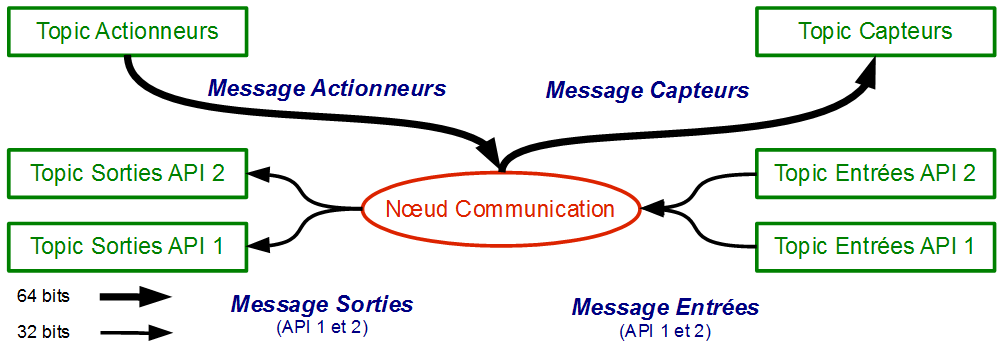
\includegraphics[scale=0.5]{Images/noeud_communication.png} 
\end{center}
\caption{Nœud \emph{Communication} avec ses topics et messages}
\label{schema_noeud_communication_topic}
\end{figure}

Comme pour le nœud \emph{Automates}, nous avons utilisé des classes pour la communication avec la couche supérieure (commande) et la couche inférieure (automates).

\subsubsection{La classe Communication\_API\_schneider}

La classe Communication\_API\_schneider permet au nœud \emph{Communication} de publier sur les topics \emph{Sorties API} 1 et 2 et de s'abonner aux topics \emph{Entrées API} 1 et 2.

\begin{center}
ATTRIBUTS
\end{center}

\begin{itemize}
\item[•] \textbf{pub\_sorties} : Objet de type Publisher. Il permettra de publier sur un topic \emph{Sorties API}.
\item[•] \textbf{sub\_entrées} : Objet de type Subscriber. Il permettra de s'abonner à un topic \emph{Entrées API}.
\item[•] \textbf{entrées\_api} : Valeurs des entrées/capteurs d'un API envoyé(e)s depuis le nœud \emph{Automates}.
\item[•] \textbf{sorties\_api} : Valeurs des sorties/actionneurs à envoyer à un API vers le nœud \emph{Automates}.
\end{itemize}

\begin{center}
MÉTHODES
\end{center}

\begin{itemize}
\item[•] \textbf{Communication\_API\_schneider(}\emph{noeud , n$^\circ$API}\textbf{)}\\
C'est le constructeur de la classe, à l'aide des paramètre \emph{noeud} et \emph{num\_API} et il permet d'initialiser \textbf{sub\_entrées} et \textbf{pub\_sorties} en les reliant au nœud \emph{Communication} qui sera déclaré dans le main. On assigne \textbf{sub\_entrées} au topic \emph{Entrées API n$^\circ$API} et \textbf{pub\_sorties} au topic \emph{Sorties API n$^\circ$API}. On initialise les attributs \textbf{entrées\_api} et \textbf{sorties\_api}.
\item[ ] 
\item[•] \textbf{Callback\_Entrees\_api(}\emph{msg}\textbf{)}\\
Cette fonction est appelée à chaque fois qu'un message de type \emph{Entrées} est publié sur le topic \emph{Entrées API n$^\circ$API} (paramètre \emph{msg}). Quand cela arrive, cette fonction actualise l'attribut \textbf{entrées\_api} de la classe.
\item[ ] 
\item[•] \textbf{publish()}\\
Cette méthode publie le message \emph{Sorties} sur le topic \emph{Sorties API n$^\circ$API} à destination du nœud \emph{Automates}.


\end{itemize}

\subsubsection{La classe Communication\_commande}

La classe Communication\_commande permet au nœud \emph{Communication} de publier sur le topic \emph{Capteurs} et de s'abonner au topic \emph{Actionneurs}.

\begin{center}
ATTRIBUTS
\end{center}

\begin{itemize}
\item[•] \textbf{pub\_capteurs} : Objet de type Publisher. Il permettra de publier sur le topic \emph{Capteurs}.
\item[•] \textbf{sub\_actionneurs} : Objet de type Subscriber. Il permettra de s'abonner au topic \emph{Actionneurs}.
\item[•] \textbf{CAPTEURS} : Valeurs de toutes les entrées/capteurs envoyé(e)s depuis le nœud \emph{Automates} après concaténation.
\item[•] \textbf{ACTIONNEURS} : Valeurs de toutes les sorties/actionneurs à envoyer aux API vers le nœud \emph{Automates} une fois qu'elles seront distribuées.
\end{itemize}

\begin{center}
MÉTHODES
\end{center}

\begin{itemize}
\item[•] \textbf{Communication\_commande(}\emph{noeud}\textbf{)}\\
C'est le constructeur de la classe, à l'aide du paramètre \emph{noeud}, il permet d'initialiser \textbf{sub\_capteurs} et \textbf{pub\_actionneurs} en les reliant au nœud \emph{Communication} qui sera déclaré dans le main. On assigne \textbf{sub\_capteurs} au topic \emph{Capteurs} et \textbf{pub\_actionneurs} au topic \emph{Actionnerus}. On initialise les attributs \textbf{CAPTEURS} et \textbf{ACTIONNEURS}.
\item[ ]
\item[•] \textbf{Concatenation\_entrees(}\emph{AP1 , AP2}\textbf{)}\\
Cette fonction permet de concaténer les entrées des API 1 et 2 reçues et stockées dans deux classes Communication\_API\_schneider \emph{AP1} et \emph{AP2}. On assigne à l'attribut \textbf{CAPTEURS} le mot de données ainsi obtenu.
\item[ ]
\item[•] \textbf{publish()}\\
Cette méthode publie le message \emph{Capteurs} sur le topic \emph{Capteurs} à destination du nœud \emph{Commande}.
\item[ ]
\item[•] \textbf{Decoupe\_sorties(}\emph{AP1 , AP2}\textbf{)}\\
Cette fonction découpe l'attribut \textbf{ACTIONNEURS} en deux parties correspondant à l'API 1 pour les données de poids faible et l'API 2 pour les données de poids fort. Le données concernant les API 1 et 2 sont alors respectivement assignées aux attributs \textbf{sorties} des paramètres \emph{AP1} et \emph{AP2} qui sont des objets de type Communication\_API\_schneider.
\item[ ]
\item[•] \textbf{Callback\_Actionneurs(}\emph{msg}\textbf{)}\\
Cette fonction est appelée à chaque fois qu'un message de type \emph{Actionneurs} est publié sur le topic \emph{Actionneurs} (paramètre \emph{msg}). Quand cela arrive, cette fonction actualise l'attribut \textbf{ACTIONNEURS} de la classe.

\end{itemize}

\subsubsection{Le main}

Dans le main (annexe \ref{annexe_main_communication}), on initialise et on déclare le nœud \textit{Communication}. Ensuite, on déclare deux objets de type Communication\_API\_schneider : \emph{AP1} et \emph{AP2} qui correspondent à la communication avec le nœud \emph{Automates}. On déclare aussi un objet de type Communication\_commande \emph{Com} qui correspond à la communication avec le nœud \emph{Commande}. Dans une boucle infinie, on concatène les entrées reçue des API puis on les publie vers la commande. Ensuite, on découpe les sorties reçues de la commande puis on les envoie vers les API. Enfin, on active les fonctions \textbf{Callback()} s'il y a des messages entrants. Cette boucle s'exécute aussi à une fréquence précise que nous détaillerons par la suite. 

\subsubsection{Validation de la communication "haute"}

Afin de valider la couche de communication, nous avons exécuté les nœud \emph{Automates} et \emph{Communication} simultanément tous en affichant les messages reçus et émis par ces 2 nœuds. Nous avons pu vérifier que le nœud \emph{Communication} recevait bien les messages du nœud \emph{Automates} et inversement. Nous avons aussi pu tester le bon fonctionnement de la concaténation en affichant les entrées des automates avant et après concaténation.

\chapter{Synthèse de commande}

Afin de commander la ligne transitique ou sa simulation à l'aide d'un même nœud ROS, nous avons tout d'abord cherché à commander la simulation seule et la ligne transitique seule avec 2 nœud ROS différents.

\section{Commande de la simulation}

Nous avons tout d'abord commencé par étudier la simulation seule. Les concepteurs de la simulation ont prévu pour la commander 3 types de messages :

\begin{itemize}
\item[ ]
\item[•] SensorState : il comprend 5 tableaux de booléens. Chaque tableau correspond aux différents types de capteurs (CPI, CP, PS, DG et DD) avec les différences que nous avons décrites précédemment (table \ref{tab:capteur_simu}).
\item[•] StopControl : il comprend 2 tableaux de booléens, un pour les actionneurs STOP et un autre pour les actionneurs GO.
\item[•] SwitchControl : il comprend 3 tableaux de booléens, les actionneurs LOCK, RD et RG. 
\item[ ]
\end{itemize}

Nous avons alors utilisé ces messages pour publier ou abonner le nœud \emph{Commande Simulation} aux topics \textit{Actionneurs\_stops}, \emph{Actionneurs\_aiguillages} et \emph{Capteurs} (figure \ref{schema_noeud_commande_simu_topic}). La simulation possède elle aussi un nœud ROS que l'on ne détaillera pas ici qui publie et s'abonne à ces topics afin de la faire évoluer.

\begin{figure}[H] 
\begin{center}
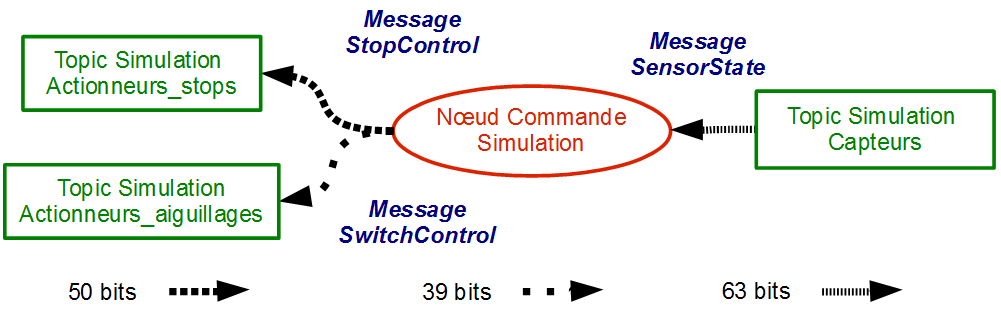
\includegraphics[scale=0.5]{Images/noeud_commande_simu_topic.png} 
\end{center}
\caption{Nœud \emph{Commande Simulation} avec ses topics et messages}
\label{schema_noeud_commande_simu_topic}
\end{figure}

Une fois la communication établie avec la simulation, nous l'avons commandée à l'aide de différents réseaux de Petri codés par mise en œuvre directe. Nous verrons des exemples de commande dans la section \ref{Validation_commande}.

\section{Commande de la ligne transitique}

Pour commander la ligne transitique seule, nous avons utilisé les messages \emph{Catpeurs} et \emph{Actionneurs} définis précédemment. Cette fois-ci le nœud \emph{Commande Ligne Transitique} publie sur le topic \emph{Actionneurs} de la ligne transitique et il est abonné au topic \emph{Capteurs} de la ligne transitique (figure \ref{schema_noeud_commande_ligne_topic}).

\begin{figure}[H] 
\begin{center}
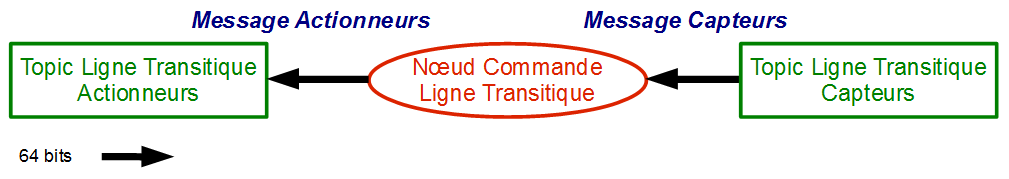
\includegraphics[scale=0.5]{Images/noeud_commande.png} 
\end{center}
\caption{Nœud \emph{Commande ligne transitique} avec ses topics et messages}
\label{schema_noeud_commande_ligne_topic}
\end{figure}

La commande est alors la même que celle de la simulation car nous souhaitons commander les deux procédés de la même façon.

\section{Commande}

Afin d'implémenter la commande finale, c'est à dire un seul nœud \emph{Commande} qui peut commander la simulation ou la ligne transitique, nous avons "fusionné" les nœuds \emph{Commande Simulation} et \emph{Commande Ligne Transitique} (figure \ref{schema_noeud_commande_gen_topic}). Maintenant, le nœud \emph{Commande} est abonné aux topics \emph{Capteurs} de la simulation et de la ligne transitique et il publie sur les topics \emph{Actionneurs\_stops}, \emph{Actionneurs\_aiguillage} de la simulation et \emph{Actionneurs} de la ligne transitique.

\begin{figure}[H] 
\begin{center}
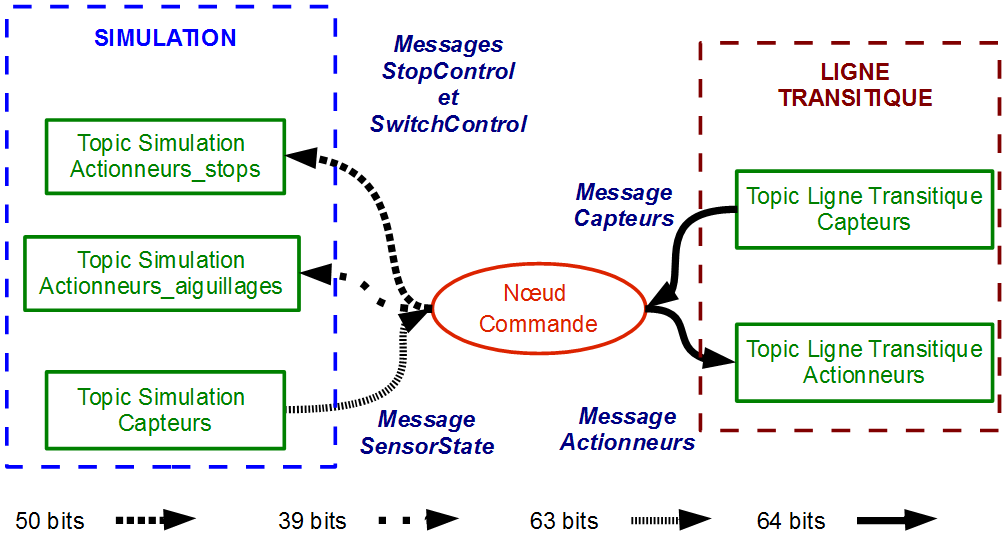
\includegraphics[scale=0.5]{Images/noeud_commande_gen_topic.png} 
\end{center}
\caption{Nœud \emph{Commande} avec ses topics et messages}
\label{schema_noeud_commande_gen_topic}
\end{figure}

\subsection{Nœud ROS \textit{Commande}}

Pour établir la communication entre le nœud \emph{Commande} et la simulation ou la ligne transitique, nous avons créé les classes Capteurs et Actionneurs.

\subsubsection{La classe Capteurs}

La classe Capteurs permet d'actualiser l'état des capteurs pour la commande que ce soit ceux de la simulation ou bien de la ligne transitique.

\begin{center}
ATTRIBUTS
\end{center}

\begin{itemize}
\item[•] \textbf{sub\_capteurs\_ligne} : Permet de s'abonner au topic \emph{Ligne Transitique Capteurs} (Subscriber).
\item[•] \textbf{sub\_capteurs\_simu} : Permet de s'abonner au topic \emph{Simulation Capteurs} (Subscriber)
\item[•] \textbf{PSx}, \textbf{DxD}, \textbf{DxG}, \textbf{CPx}, \textbf{CPIx} : Tableaux contenant les valeurs des différents types de capteurs qui seront mis à jour pendant l'exécution du nœud.
\item[•] \textbf{SIMULATION}, \textbf{LIGNE} : Indicateurs permettant de savoir si la commande communique avec la ligne transitique (\textbf{LIGNE}=1 et \textbf{SIMULATION}=0) ou avec la simulation (\textbf{SIMULATION}=1 et \textbf{LIGNE}=0).
\end{itemize}

\newpage

\begin{center}
MÉTHODES
\end{center}

\begin{itemize}
\item[•] \textbf{Capteurs(}\emph{noeud}\textbf{)}\\
C'est le constructeur de la classe, il assigne les attributs \textbf{sub\_capteurs\_ligne} et \textbf{sub\_capteurs\_simu} à leurs topics respectifs. Il initialise aussi tous les tableaux des capteurs ainsi que \textbf{SIMULATION} et \textbf{LIGNE} à 0.
\item[ ] 
\item[•] \textbf{Actualiser(}\emph{PS , DD , DG , CP , CPI}\textbf{)}\\
Cette fonction actualise les capteurs déclarés dans le main pour la commande faite par RdP ou MEF.
\item[ ] 
\item[•] \textbf{Callback\_capteurs\_ligne(}\emph{msg}\textbf{)}\\
Cette fonction actualise les attributs \textbf{PSx}, \textbf{DxD}, \textbf{DxG}, \textbf{CPx} et \textbf{CPIx} de la classe Capteurs lorsque la ligne transitique est active.
\item[ ] 
\item[•] \textbf{Callback\_capteurs\_simulation(}\emph{msg}\textbf{)}\\
Cette fonction actualise les attributs \textbf{PSx}, \textbf{DxD}, \textbf{DxG}, \textbf{CPx} et \textbf{CPIx} de la classe Capteurs lorsque la simulation est active.
\item[ ] 
\item[•] \textbf{Actualiser\_PSx(}\emph{CAPTEURS}\textbf{)}, \textbf{Actualiser\_DxD(}\emph{CAPTEURS}\textbf{)}, \textbf{Actualiser\_DxG(}\emph{CAPTEURS}\textbf{)}, \textbf{Actualiser\_CPx(}\emph{CAPTEURS}\textbf{)}, \textbf{Actualiser\_CPIx(}\emph{CAPTEURS}\textbf{)}\\
Ces méthodes permettent d'actualiser les tableaux de capteurs de la classe à partir du message \emph{CAPTEURS} reçu depuis la ligne transitique.
\item[ ] 
\item[•] \textbf{MASK(}\emph{registre , numero\_bit}\textbf{)}\\
Cette fonction n'est pas une méthode de la classe mais elle est très utile pour l'actualisation des capteurs lorsqu'ils sont envoyés par la ligne transitique. Comme nous l'avons vu précédemment, elle permet de récupérer un seul bit d'un mot de données.
\end{itemize}

\subsubsection{La classe Actionneurs}

La classe Actionneurs permet d'envoyer les valeurs des actionneurs déterminées par la commande que soit pour la simulation ou bien pour la ligne transitique.

\begin{center}
ATTRIBUTS
\end{center}



\begin{itemize}
\item[•] \textbf{pub\_actionneurs\_ligne} : Permet de publier sur le topic \emph{Ligne Transitique Actionneurs} (Publisher).
\item[•] \textbf{pub\_actionneurs\_simu\_aguillages} : Permet de publier sur le topic \emph{Simulation Actionneurs\_aiguillages} (Publisher).
\item[•] \textbf{pub\_actionneurs\_simu\_stops} : Permet de publier sur le topic \emph{Simulation Actionneurs\_stops} (Publisher).
\item[•] \textbf{Actionneurs\_ligne} : Mot de données correspondant aux actionneurs à destination de la ligne transitique.
\item[•] \textbf{actionneurs\_simulation\_Stop} : Mot de données correspondant aux actionneurs stops à destination de la simulation.
\item[•] \textbf{actionneurs\_simulation\_Aguillages} : Mot de données correspondant aux actionneurs aiguillages à destination de la simulation.
\end{itemize}

\begin{center}
MÉTHODES
\end{center}


\begin{itemize}
\item[•] \textbf{Actionneurs(}\emph{noeud}\textbf{)}\\
C'est le constructeurs de la classe, il assigne les attributs \textbf{pub\_actionneurs\_ligne}, \textbf{pub\_actionneurs\_\\simu\_aguillages} et \textbf{pub\_actionneurs\_simu\_stops} à leurs topics respectifs. Il initialise aussi \textbf{Actionneurs\_ligne}, \textbf{actionneurs\_simulation\_Stop} et \textbf{actionneurs\_simulation\_Aguillages} à 0.
\item[ ] 
\item[•] \textbf{Envoyer(}\emph{STx , RxD , RxG , Vx , Dx , PIx}\textbf{)}\\
Cette méthode permet de mettre à jour les actionneurs de la simulation et de la ligne transitique.
\item[ ] 
\item[•] \textbf{publish\_actionneurs\_ligne()}\\
Cette méthode publie le message \emph{Actionneurs} sur le topic \emph{Ligne Transitique Actionneurs}
\item[ ] 
\item[•] \textbf{publish\_actionneurs\_simulation()}\\
Cette méthode publie les messages \emph{StopControl} et \emph{SwtichControl} sur les topics \emph{Simulation Actionneurs\_stops} et \emph{Simulation Actionneurs\_aiguillages}.
\item[ ] 
\item[•] \textbf{Ecrire\_ligne\_STx(}\emph{STx}\textbf{)}, \textbf{Ecrire\_ligne\_RxD(}\emph{RxD}\textbf{)}, \textbf{Ecrire\_ligne\_RxG(}\emph{RxG}\textbf{)},\\
\textbf{Ecrire\_ligne\_PIx(}\emph{PIx}\textbf{)}, \textbf{Ecrire\_ligne\_Vx(}\emph{Vx}\textbf{)}, \textbf{Ecrire\_ligne\_Dx(}\emph{Dx}\textbf{)}\\
Ces méthodes permettent de modifier l'attribut \textbf{Actionneurs\_ligne} en fonction des tableaux d'actionneurs venant de la commande (main).
\item[ ] 
\item[•]  \textbf{WRITE(}\emph{registre , donnee, numero\_bit}\textbf{)}\\
Cette fonction n'appartient pas non plus à la classe Actionneurs mais elle est très utile pour écrire les valeurs des actionneurs un à un pour la ligne transitique. Comme énoncé précédemment, elle permet de modifier un seul bit dans un mot de données.
\end{itemize}

\subsubsection{Fonctions supplémentaires}

Afin de simplifier au maximum le main du nœud \emph{Commande}, nous avons créé les fonctions suivantes :

\begin{itemize}
\item[•] \textbf{Initialisation(}\emph{PSx , DxD , DxG , CPx , CPIx , STx , RxD , RxG , Vx , Dx , PIx}\textbf{)}\\
Cette fonction initialise tous les capteurs et actionneurs nécessaires à la commande déclarés dans le main.
\item[ ] 
\item[•] \textbf{Deplacer\_navettes(}\emph{Actionneurs , STx , RxD , RxG , Vx , Dx , PIx , numero\_stop}\textbf{)}\\
Cette fonction permet de déplacer les navettes devant n'importe quel stop de la ligne transitique sur la simulation pour choisir la position initiale des navettes. Sur la ligne transitique réelle, on peut disposer les navettes à la main.
\item[ ] 
\item[•] \textbf{Mode\_ligne(}\emph{Actionneurs , STx , RxD , RxG , Vx , Dx , PIx}\textbf{)}\\
Cette fonction permet de mettre la simulation dans la même configuration que la ligne transitique. Durant notre projet, nous n'avons commandé que les automates 1 et 2, nous avons donc bloqué les aiguillages 3 et 10 en position gauche. Cette fonction fait la même chose lorsque l'on commande la simulation et que l'on souhaite que celle-ci soit dans la même configuration que la ligne réelle.
\item[ ] 
\item[•] \textbf{Afficher\_capteurs(}\emph{PSx , DxD , DxG , CPx , CPIx}\textbf{)}, \textbf{Afficher\_actionneurs(}\emph{STx , RxD , RxG , Vx , Dx , PIx}\textbf{)}, \textbf{Afficher\_marquage\_RdP(}\emph{M , nombre\_places}\textbf{)}\\ 
Ces fonction permettent d'afficher en temps réel les valeurs de tous les capteurs, actionneurs et du marquage du RdP de la commande pour vérifier le bon fonctionnement de la commande.
\end{itemize}

\subsubsection{Le main}

C'est dans le main (annexe \ref{annexe_packages_commande_main}) que l'on peut alors choisir la commande à effectuer. Premièrement on déclare et on initialise le nœud \emph{Commande}. Ensuite, on déclare un objet de type Actionneurs et un objet de type Capteurs. Nous avons choisi une fréquence de 25Hz pour chaque itération de la boucle infinie de commande, il faut alors que la fréquence du nœud \emph{Communication} soit supérieure à cette fréquence et celle du noeud \emph{Automates} doit être supérieure à la fréquence du nœud \emph{Communication}. Ainsi la commande ne peut pas évoluer plus rapidement que les messages ne sont transmis à travers les nœud \emph{Communication} et \emph{Automates}.\\

On déclare alors les tableaux du marquage du RdP, des capteurs et des actionneurs puis on les initialise. On a ensuite une boucle infinie dans laquelle on déplace les navettes et on configure la simulation si besoin. Toujours dans la boucle, on actualise alors les valeurs des capteurs, et on envoie les nouvelles valeurs des actionneurs données la mise en œuvre du réseau de Petri. Enfin, on lance les fonctions Callback s'il y a eu des messages entrants et on synchronise la boucle sur la fréquence choisie.


\newpage
\section{Validation de la commande \label{Validation_commande}}

Afin de valider le fonctionnement du nœud \emph{Commande} nous avons tout d'abord implémenté des commandes simples modélisées par des MEF mais il était compliqué d'utiliser plusieurs navettes avec cette méthode. Nous avons alors utilisé des réseaux de Petri pour commander plusieurs navettes en parallèle.

\subsection{Test de la simulation}

Afin de valider notre commande sous ROS ainsi que la simulation conçue sur V-REP nous avons choisi de faire un réseau de Petri permettant de faire évoluer les navettes sur l'ensemble de la ligne sur la simulation (figures \ref{RdP_1234_simu}, \ref{RdP_5678_simu} et \ref{RdP_9101112_simu}).\\

Nous avons choisi pour objectif que lorsqu'une navette arrive devant un aiguillage et que 2 directions s'offrent à elle, l'aiguillage doit changer son orientation avant de faire circuler la navette. Ainsi, chaque navette ira dans la direction opposée à celle que la dernière navette a emprunté. De cette façon, on distribue au maximum les navettes sur tous les rails. Lorsqu'une navette arrive sur un aiguillage et qu'elle n'a pas de choix de direction, l'aiguillage doit se mettre dans la bonne position pour la laisser passer.\\

Nous avons alors ajouté des places pour modéliser la disponibilité d'un aiguillage pour éviter qu'un aiguillage de change de position lorsqu'une navette n'a pas fini de passer (places rouges). Pour simplifier la représentation du réseau de Petri nous l'avons décomposé en plusieurs blocs correspondant aux différentes trajectoires de navettes possibles.\\

Pour la mise en œuvre, nous avons fusionné les transition vertes qui avaient les même numéros et nous avons aussi fusionné les places rouges qui apparaissaient plusieurs fois avec le même numéro. Certains aiguillages sont parfois libérés plus tard que d'autres en fonction du trajet emprunté par la maquette.\\

Implémenter cette commande nous a permis de détecter certains problèmes sur la simulation que nous avons pu rectifier. Certains capteurs n'étaient pas bien positionnés ce qui entrainait des blocages pendant l'exécution de la commande. Tester notre commande sur la simulation nous a aussi permis de détecter des erreurs que nous avions commis dans la modélisation ou dans le codage sans qu'elles n'aient été fatales pour les navettes de la ligne transitique.\\

Pour cette commmande, nous n'avons pas utilisé la fonction Mode\_Ligne() car nous avons utilisé la totalité de la ligne transitique. Cependant, nous avons disposé les navettes devant deux stops différents (ST12 et ST24) pour correspondre avec le marquage initial du RdP.\\

\vspace{5cm}

\begin{figure}[H] 
\begin{center}
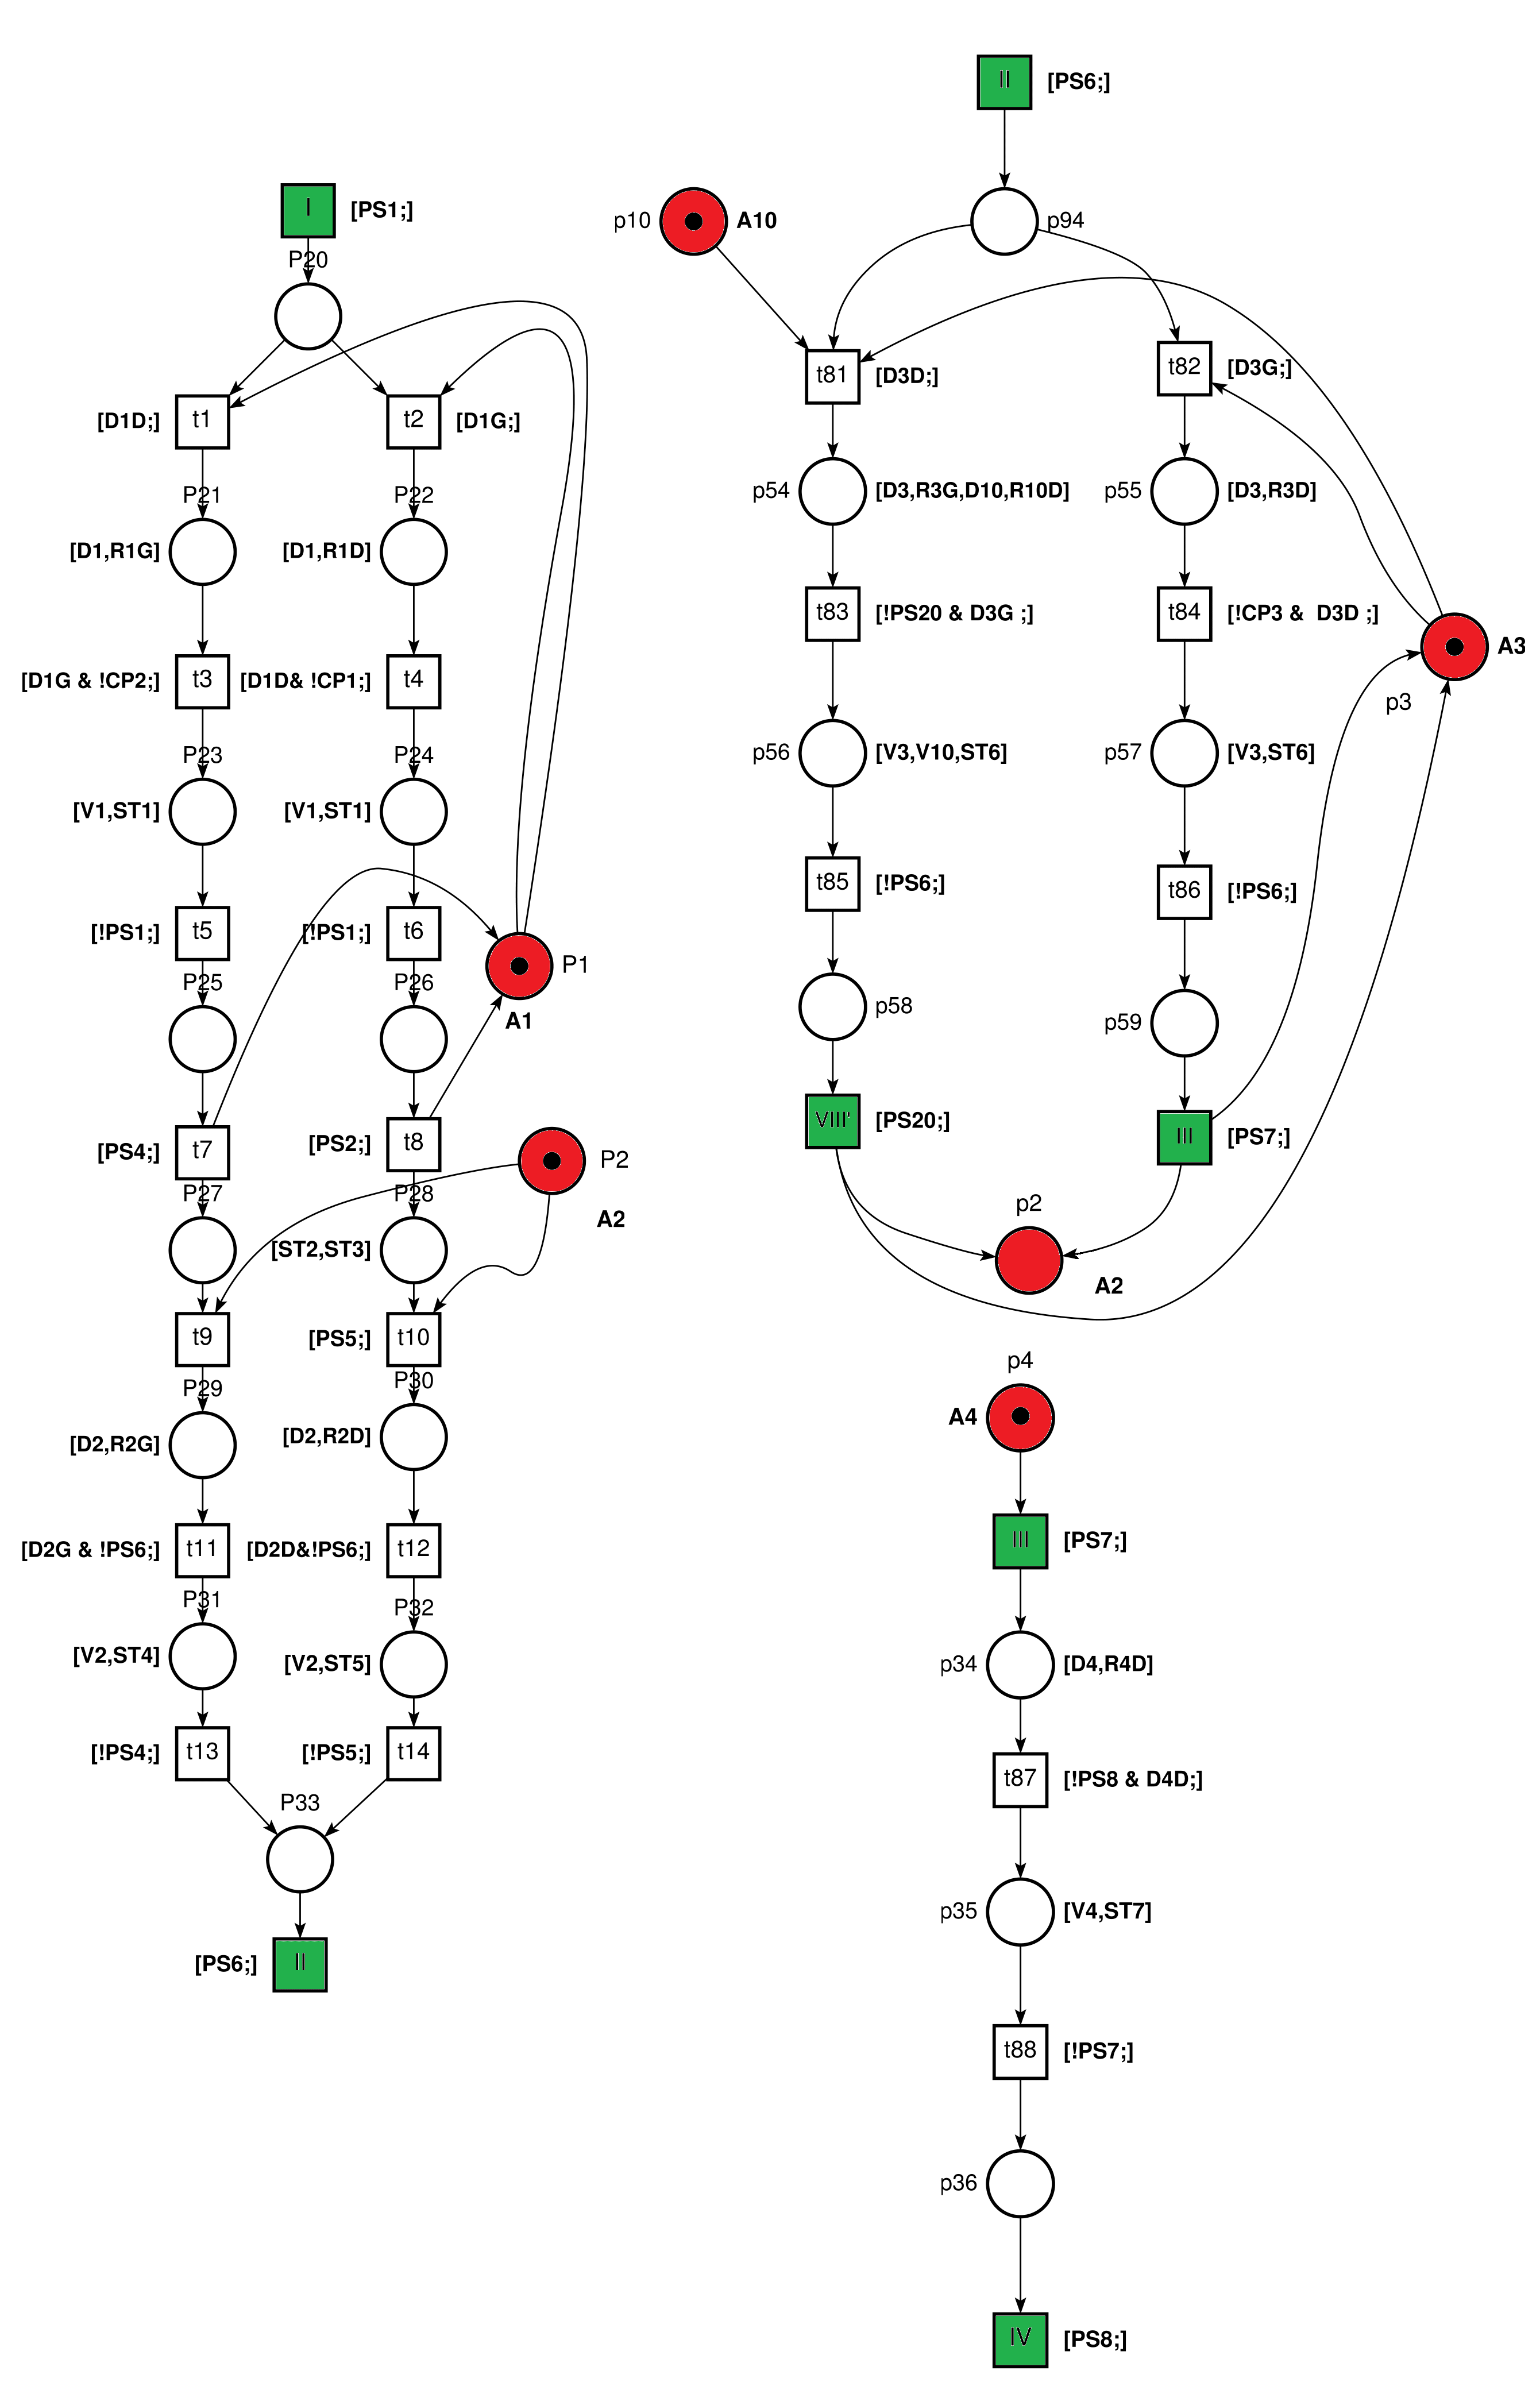
\includegraphics[scale=0.2]{RdP/RDP1.png} 
\end{center}
\caption{Réseau de Petri de la commande sur la simulation de la ligne transitique, commande pour des navettes passant par les aiguillages A1, A2, A3 puis A4 ou A10}
\label{RdP_1234_simu}
\end{figure}

\begin{figure}[H] 
\begin{center}
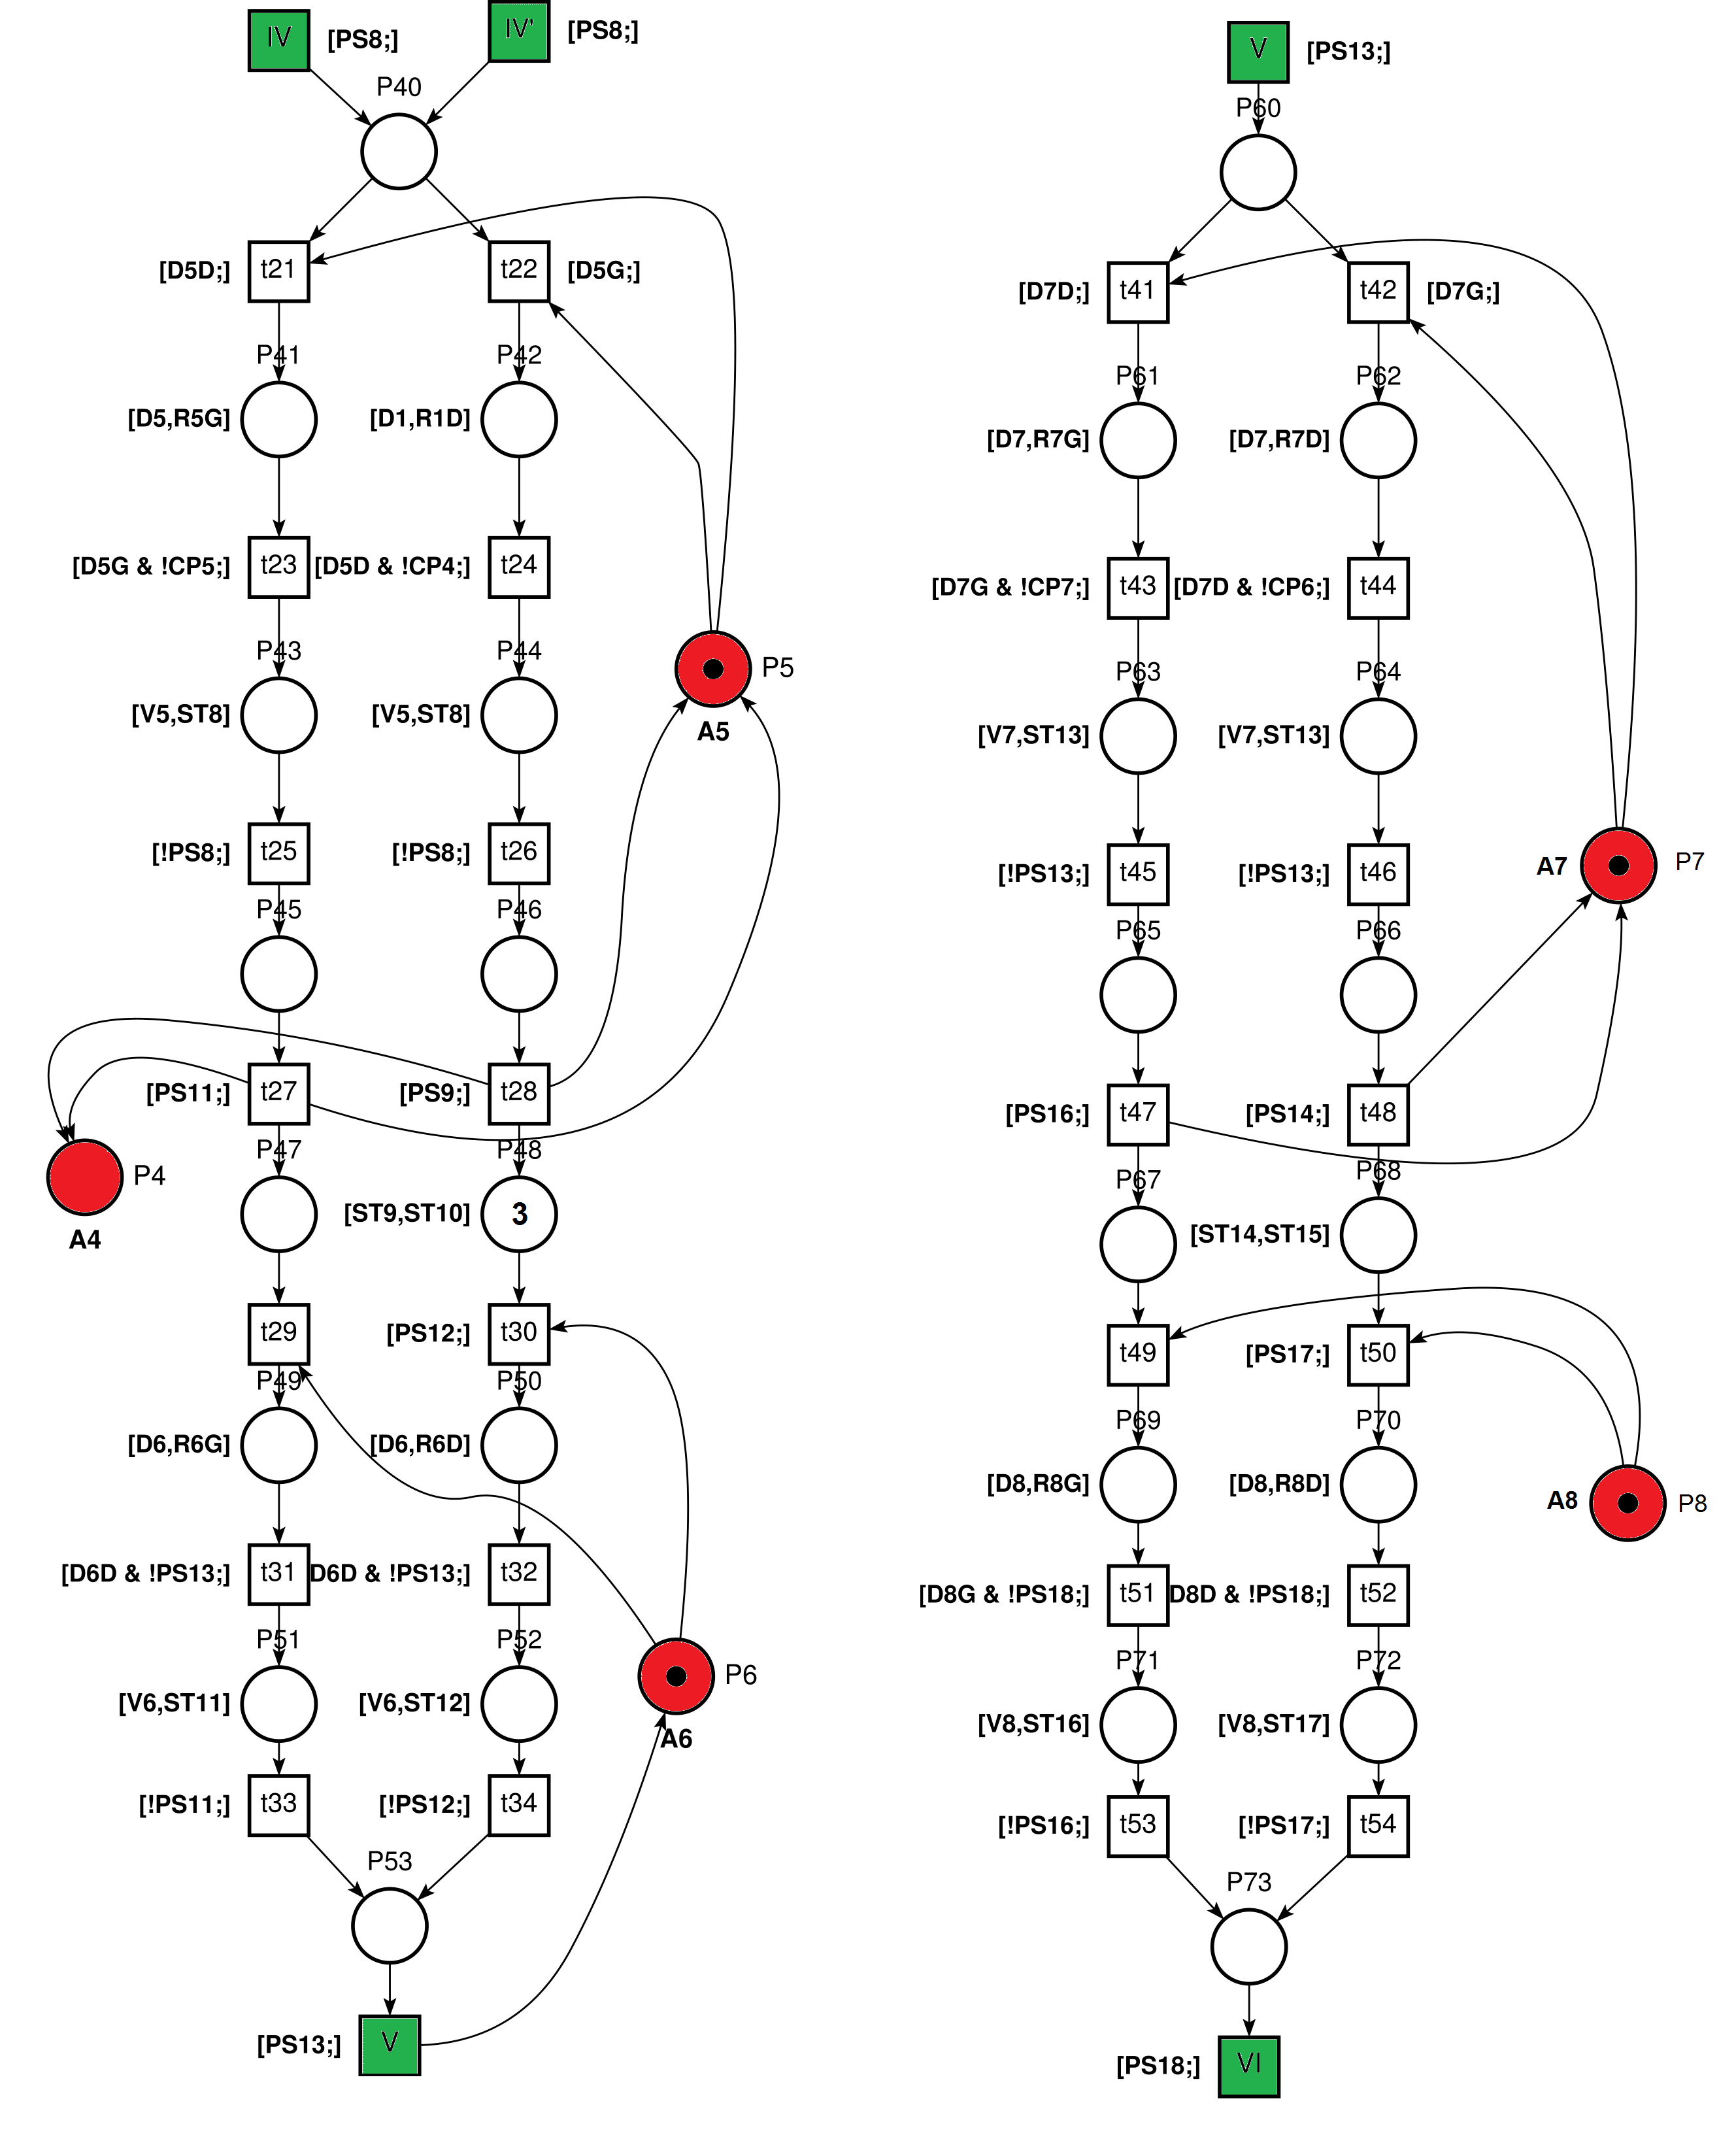
\includegraphics[scale=0.25]{RdP/RDP2.png} 
\end{center}
\caption{Réseau de Petri de la commande sur la simulation de la ligne transitique, commande pour des navettes passant par les aiguillages A5, A5, A7 et A8}
\label{RdP_5678_simu}
\end{figure}

\begin{figure}[H] 
\begin{center}
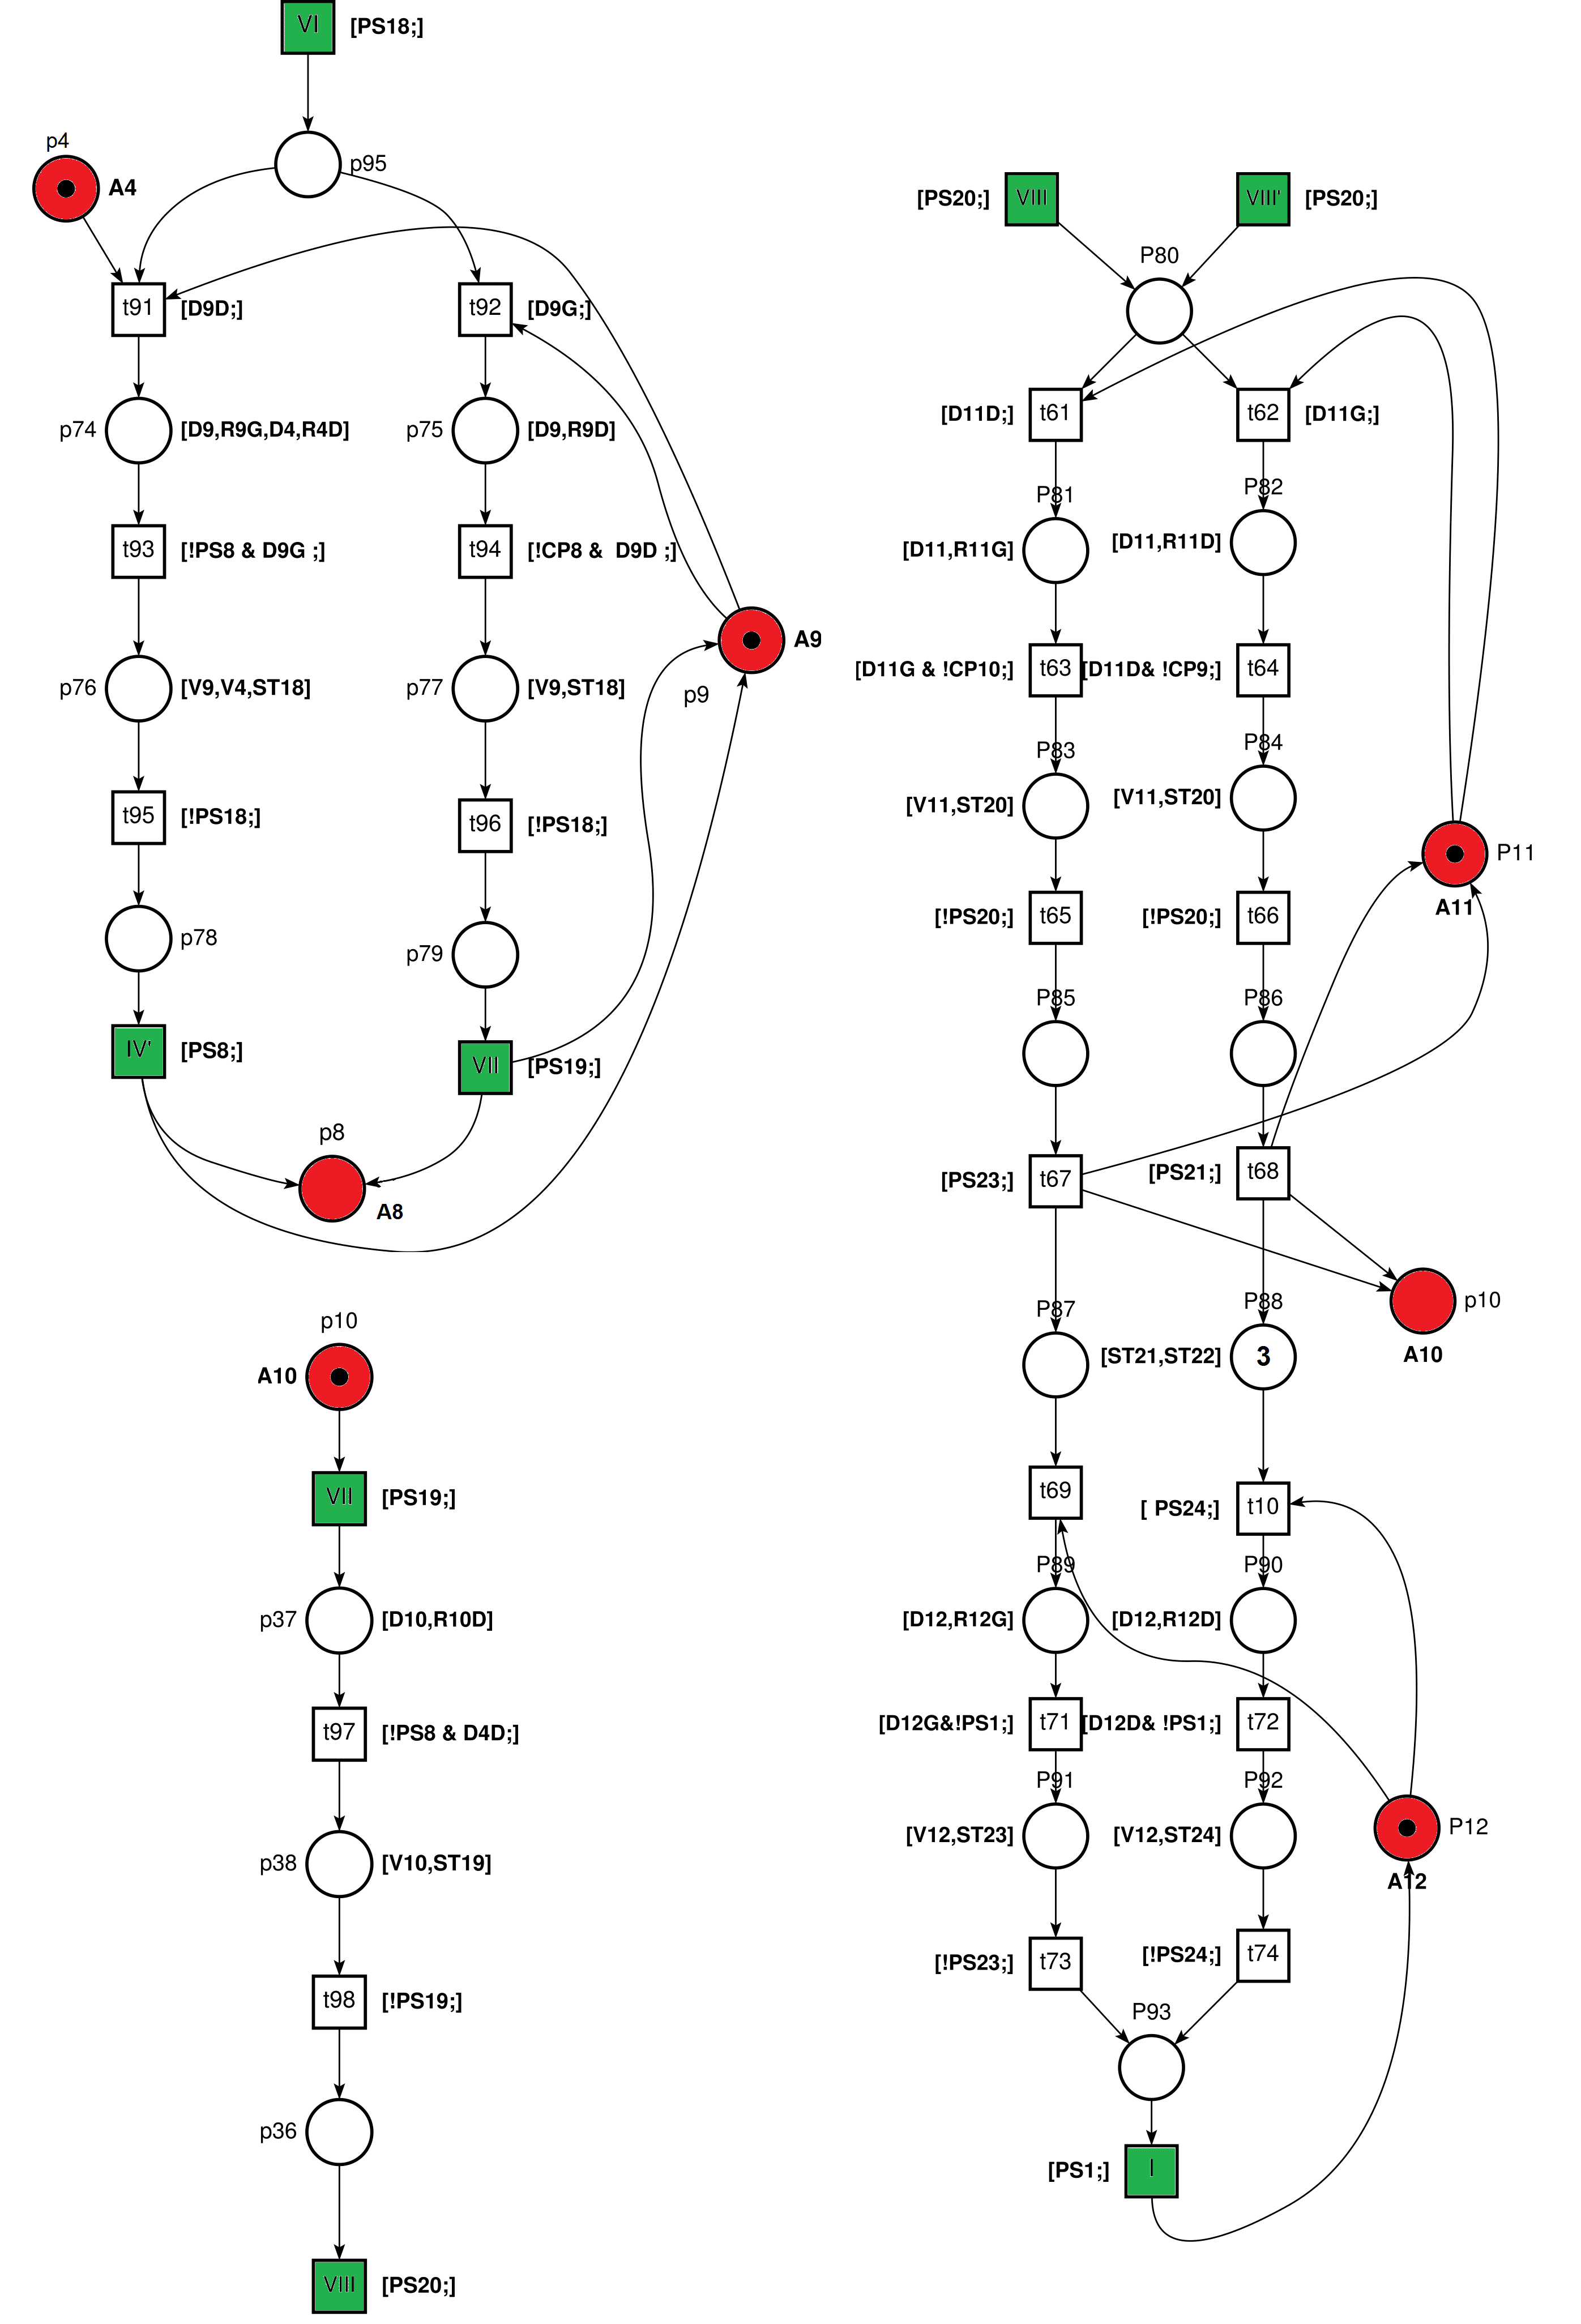
\includegraphics[scale=0.2]{RdP/RDP3.png} 
\end{center}
\caption{Réseau de Petri de la commande sur la simulation de la ligne transitique, commande pour des navettes passant par les aiguillages A9 et A4 ou A9, A10, A11 et A12}
\label{RdP_9101112_simu}
\end{figure}



\subsection{Test de la ligne transitique}

Dans notre cas, nous ne pouvions commander que les automates 1 et 2 et donc les aiguillages 1, 2, 11 et 12. Afin de tester une commande à la fois sur la simulation et sur la ligne transitique nous avons gardé la commande précédente en supprimant tous les autres aiguillages (figure \ref{RdP_lign_simu}).\\

Nous avons utilisé cette fois la fonction Mode\_Ligne() pour mettre la simulation dans la même configuration que la ligne transitique (A3 et A10 à gauche).\\



\begin{figure}[H] 
\begin{center}
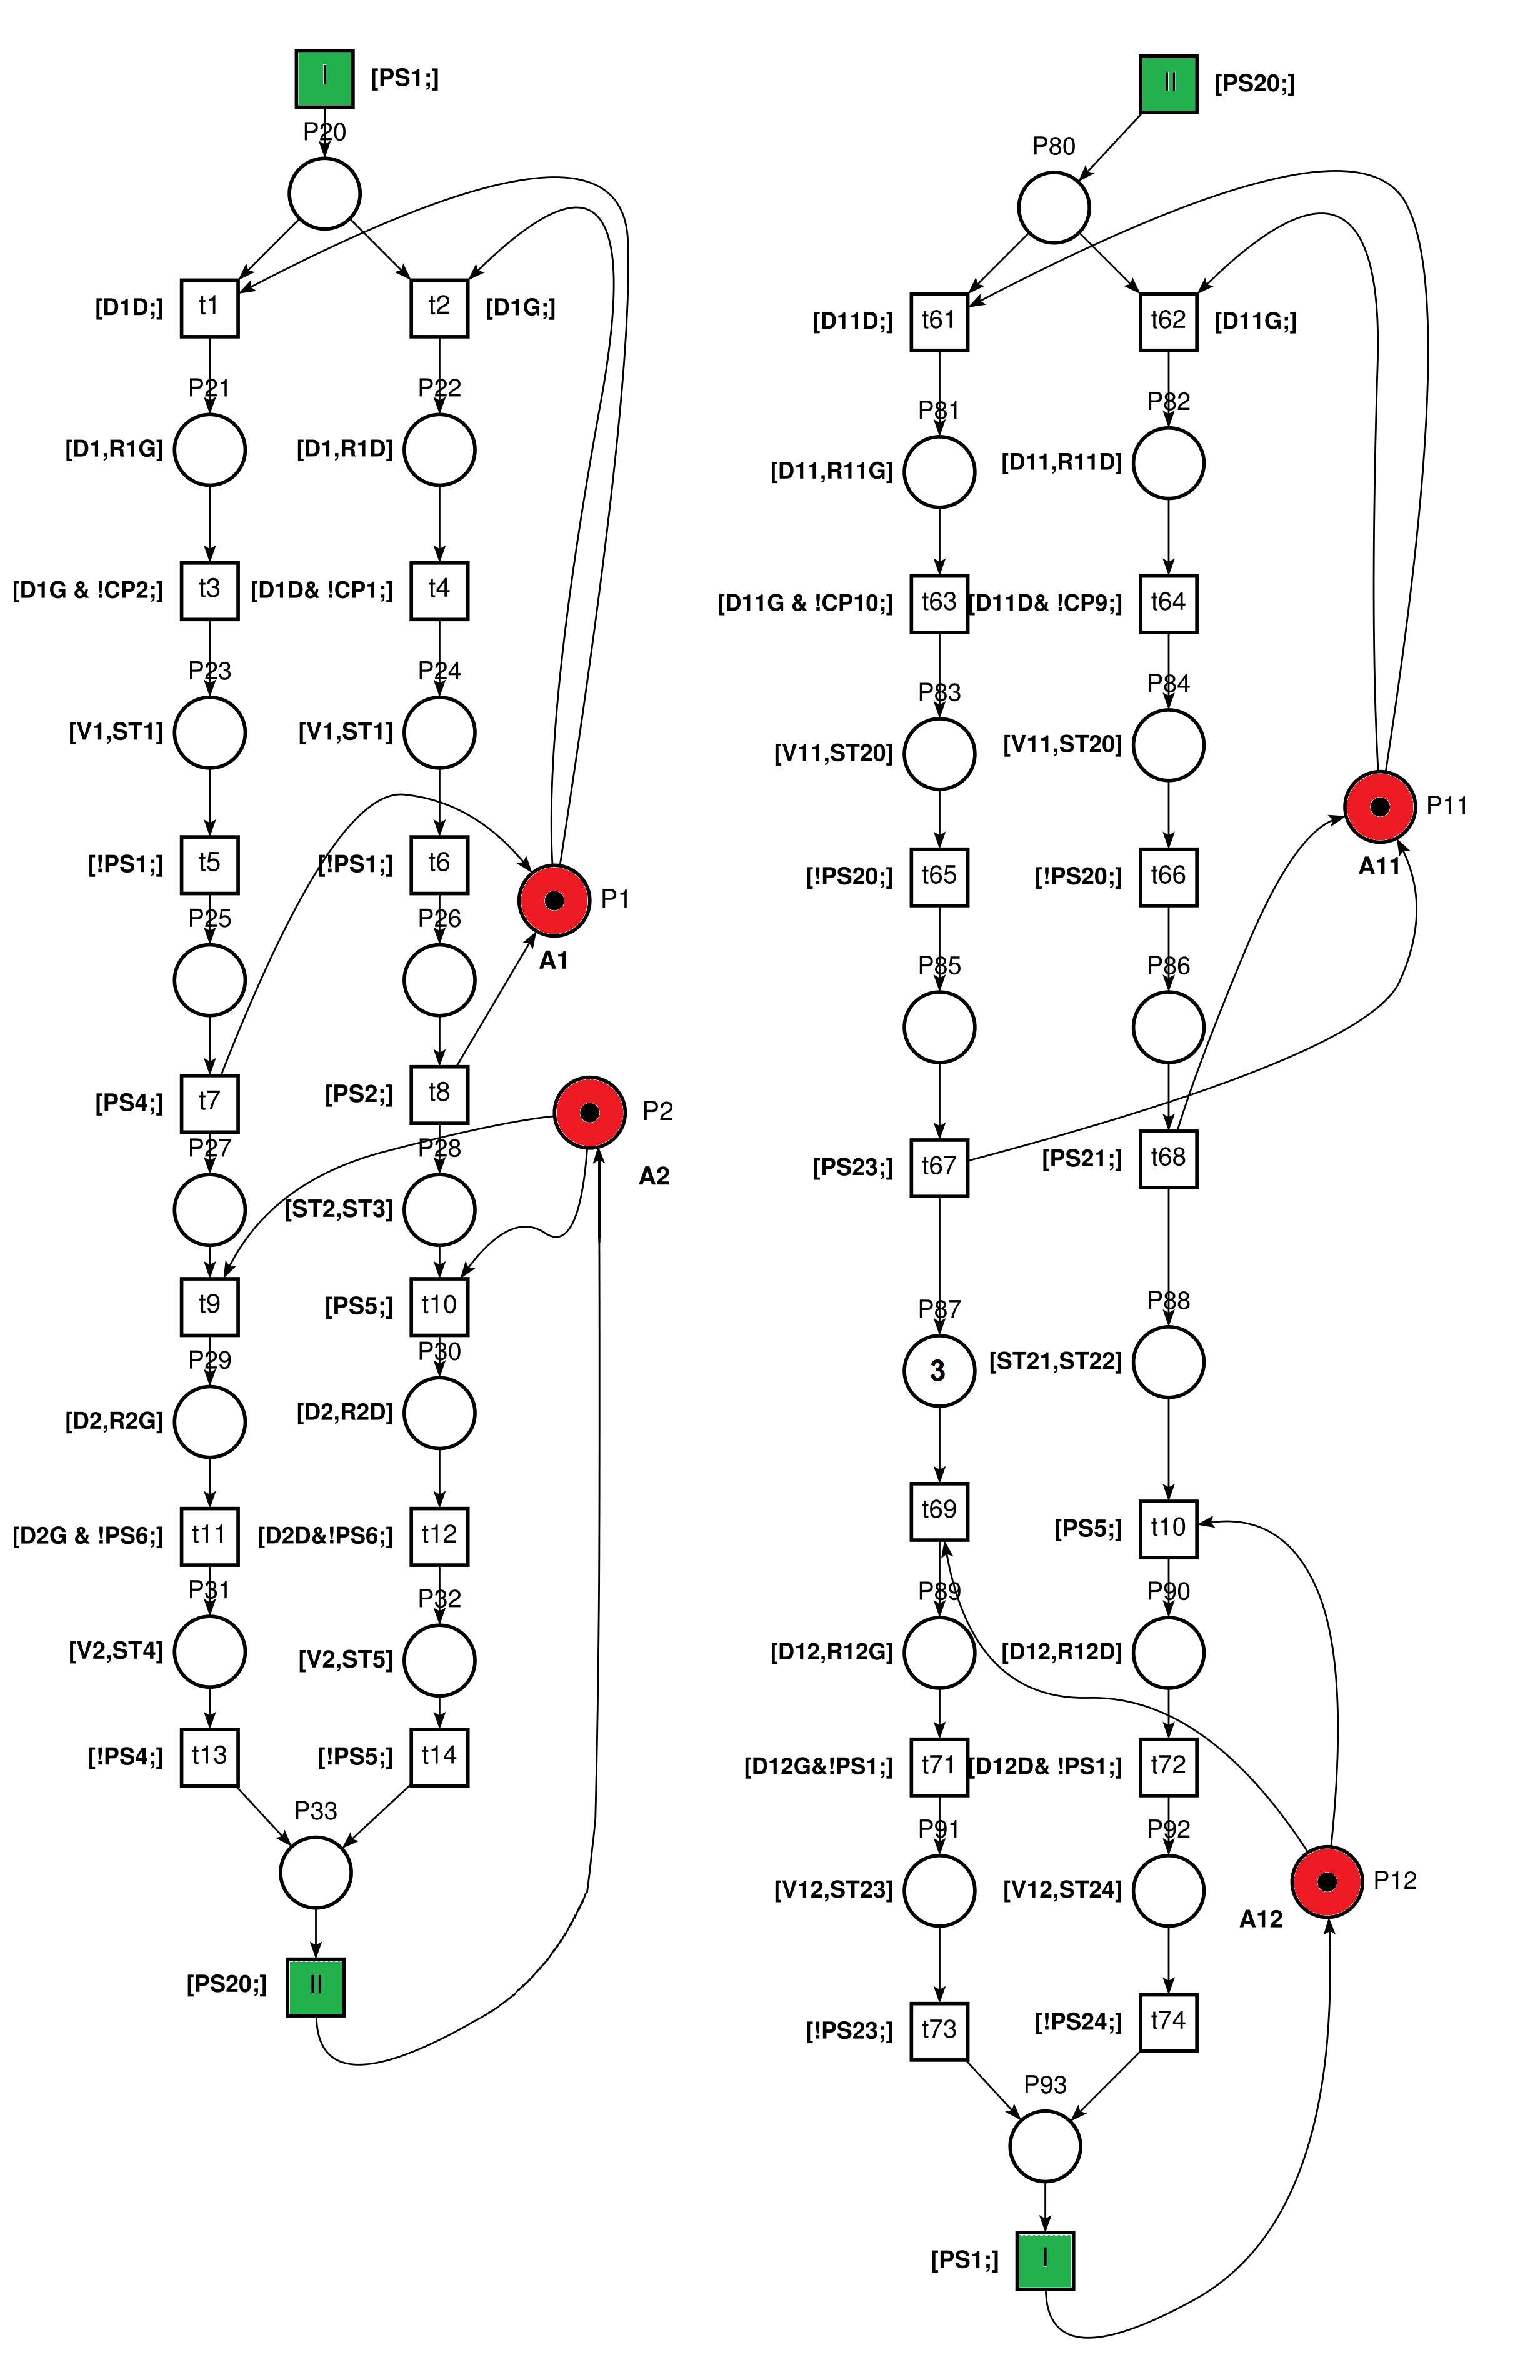
\includegraphics[scale=0.2]{RdP/RDP4.png} 
\end{center}
\caption{Réseau de Petri de la commande des aiguillages 1, 2, 11 et 12 sur la ligne transitique}
\label{RdP_lign_simu}
\end{figure}



\newpage
\addcontentsline{toc}{section}{Conclusion}
\chapter*{Conclusion}


Durant ce projet, tout d'abord, nous avons appris à utiliser la plateforme ROS et nous nous sommes perfectionnés dans le langage C++ et en informatique en général. Nous avons découvert le fonctionnement d'une ligne transitique et comment est ce qu'il faut s'y prendre pour la commander.\\

Nous sommes parvenus à établir un pont de communication avec la ligne transitique avec l'outil ROS ce qui nous a permis ensuite d'implémenter différentes commandes sur la simulation et sur la ligne. Ces commandes nous ont permis de valider noter travail ainsi que celui des concepteurs la simulation. En effet, nous avons dû appliquer certains changements sur la simulation pour améliorer son fonctionnement.\\

Il faudrait maintenant établir la communication avec les autres secteurs de la ligne transitique afin de pouvoir implémenter des commandes sur l'ensemble de la ligne et pouvoir profiter de toutes ces zones.\\

Enfin, il faudrait finir de concevoir la simulation pour qu'elle prennent en compte la totalité des actionneurs présents sur la ligne transitique ce qui n'est pas encore le cas. Ainsi, la maquette serait opérationnelle et pourrait alors accueillir des TP.

\newpage
\addcontentsline{toc}{section}{Bibliographie}
\chapter*{Bibliographie}\label{biblio}



\begin{itemize}
\item[ \textbf{[1]}] ABIVEN Cédric, CARDONE Grégoire, GAO Shengheng. \textit{Commande d'une ligne transitique MONTRAC}. Rapport de TER, Master 1 Électronique Électrotechnique Automatique, Ingénierie des Sytèmes Temps-Réel. Toulouse : Université Paul Sabatier, 2015.
\item[ ]
\item[ \textbf{[2]} ] ANTONIUTTI Emilie, BERTIN Thibault, DEMMER Simon, LE BIHAN Clément. \textit{Commande et Simulation d'un réseau de transport d'un système de production}. Rapport de Projet Long, GEA CDISC. Toulouse : ENSEEIHT, 2016.\\
Disponible sur <\verb!https://github.com/ClementLeBihan/CelluleFlexible/blob/master/Livrables/R!\\
\verb!apport_Projet_Long!> (Consulté le 26.05.2016)
\item[ ]
\item[ \textbf{[3]} ] ANTONIUTTI Emilie, BERTIN Thibault, DEMMER Simon, LE BIHAN Clément. \textit{Simulation de la ligne transitique MONTRAC}. Code source (GIT). Toulouse : ENSEEIHT, 2016.\\
Disponible sur <\verb!https://github.com/ClementLeBihan/CelluleFlexible!> (Consulté le 26.05.2016)
\item[ ]
\item[ \textbf{[4]} ] GORRY POLLET Alexandra. \textit{Commande d’une cellule flexible de production robotisée}. Rapport de stage, IUT Génie Électrique et Informatique Industrielle. Toulouse : Université Paul Sabatier, 2015.
\item[ ]
\item[ \textbf{[5]} ] AIP-PRIMECA. \textit{Pôle AIP-PRIMECA Toulouse}.\\
Disponible sur <\verb!http://aip-primeca.ups-tlse.fr/!> (Consulté le 26.05.2016)
\item[ ]
\item[ \textbf{[6]} ] Robot Operating System. \textit{ROS}.\\
Disponible sur <\verb!http://www.ros.org/!> (Consulté le 26.05.2016)
\item[ ]
\item[ \textbf{[7]} ] V-REP. \textit{v-rep virtual robot experimentation platform}.\\
Disponible sur <\verb!http://www.coppeliarobotics.com/!> (Consulté le 26.05.2016)
\item[ ]
\item[ \textbf{[8]} ] OPENCLASSROOMS. \textit{Programmez avec le langage C++}.\\
Disponible sur <\verb!https://openclassrooms.com/courses/programmez-avec-le-langage-c!> (Consulté le 26.05.2016)
\item[ ]
\item[ \textbf{[9]} ] LIBMODBUS. \textit{A Modbus library for Linux, Mac OS X, FreeBSD, QNX and Win32}.\\
Disponible sur <\verb!http://libmodbus.org/!> (Consulté le 26.05.2016)
\item[ ]
\end{itemize}

\newpage

\appendix
\addtocontents{toc}{\protect\setcounter{tocdepth}{0}}

\chapter{Guide d'utilisation de ROS\label{annexe_ROS}}

\section{Installation}

L'installation du ROS ne peux se faire que sur une machine virtuelle, Ubuntu par exemple. Vous êtes prêts à commencer l'installation? Avant de commencer, il faut Configurer votre machine afin qu'il accepte les logiciels depuis ros.org, pour cela, vous devez lancer la commande suivante sur un terminal.
\begin{Verbatim}
  $ sudo sh -c 'echo "deb http://packages.ros.org/ros/ubuntu quantal
    main" > /etc/apt/sources.list.d/ros-latest.list'
\end{Verbatim}
Il est conseillé de configurer les touches de votre machine. 
\begin{Verbatim}
  $ sudo apt-key adv --keyserver hkp://ha.pool.sks-keyservers.net:80 --recv-key 0xB01FA116
\end{Verbatim}
Il serait aussi préférable de mettre à jour le logiciel pour éviter les problèmes avec les bibliothèques.
\begin{Verbatim}
  $ sudo apt-get update
  $ echo "source /opt/ros/jade/setup.bash" >> ~/.bashrc
  $ source ~/.bashrc
\end{Verbatim}

\section{Création un environnement de travail}

Avant de commencer écrire n'importe quel code sur ROS, il faut d'abord créer votre environnement du travail "workspace"
\begin{Verbatim}
  $ mkdir -p ~/catkin_ws/src
  $ cd ~/catkin_ws/src
  $ catkin_init_workspace 
\end{Verbatim}

\section{Création de packages}
Le package est un répertoire qui contient les nœuds, les librairies externes, des données, des fichiers de configuration et le fichier xml. 

D'abord vous aller vous rendre au le fichier source dans l'espace de travail catkin (workspace), vous allez créer maintenant un package nommé "premier$\_$programme" qui dépend de std$\_$msgs, roscpp et Rospy : 
  
\begin{Verbatim}
  $ cd ~/catkin_ws/src
  $ catkin_create_pkg premier_programme std_msgs rospy roscpp
\end{Verbatim}

Cela va créer un dossier premier$\_$programme qui contient un package.xml et un CMakeLists.txt , qui vont être remplis avec les informations que vous avez donné à catkin\_create$\_$pkg. catkin$\_$create$\_$pkg exige que vous lui donniez un package$\_$name et éventuellement une liste des dépendances.
Si on ouvre le fichier package.xml on se retrouve avec : 

\begin{Verbatim}
  ...
  <buildtool_depend>catkin</buildtool_depend>
  <build_depend>roscpp</build_depend>
  <build_depend>rospy</build_depend>
  <build_depend>std_msgs</build_depend>
  ...
  <license>TODO</license> 
  ...
\end{Verbatim}
Les dépendances peuvent maintenant être examinées avec l'outil rospack.\\\\
Exemple : 
\begin{Verbatim}
   $ rospack depends1  rospy
\end{Verbatim}

Cela dervait générer: 

\begin{Verbatim}
  genpy
  rosgraph
  rosgraph_msgs
  roslib
  std_msgs
\end{Verbatim}

Puisque la majorités des composants ROS utilisent la licence  $BSD$ il faut la modifier. La version finale de votre package serai comme ceci :\\
\begin{Verbatim}
  <?xml version="1.0"?>
  <package>
  <name>premier_programme</name>
  <version>0.1.0</version>
  <description>The premier_programme package</description>
  <maintainer email="you@yourdomain.tld">Your Name</maintainer>
  <license>BSD</license>
  <url type="website">http://wiki.ros.org/premier_programme</url>
  <author email="you@yourdomain.tld">Jane Doe</author>
  <buildtool_depend>catkin</buildtool_depend>
  <build_depend>roscpp</build_depend>
  <build_depend>rospy</build_depend>
  <build_depend>std_msgs</build_depend>
  <run_depend>roscpp</run_depend>
  <run_depend>rospy</run_depend>
  <run_depend>std_msgs</run_depend>
  </package>
\end{Verbatim}

\section{Les makefiles}

Après avoir créé votre environnement du travail et vos packages, vous avez besoin maintenant de configurer le Cmakefile qui vas générer un makefile dans le fichier build, afin d'exécuter l'ensemble des actions souhaitées. Retournez donc au fichier package.xml, vous trouverez :

\begin{Verbatim}
  <buildtool_depend>catkin</buildtool_depend>
\end{Verbatim}  

On crée  mon$\_$pkg et on ajoute une dépendance sur Rospy de sorte que vous pouvez utiliser dans ce code

\begin{Verbatim}  
  $ cd ~/catkin_ws/src
  $ catkin_create_pkg mon_pkg message_generation rospy
\end{Verbatim}  

Le fichier Camkelists devrait contenir les éléments suivants :

\begin{Verbatim} 
  <build_depend>message_generation</build_depend>
\end{Verbatim} 

\begin{Verbatim}  
  cmake_minimum_required(VERSION 2.8.3)
  project(mon_pkg)

  find_package(catkin REQUIRED COMPONENTS message_generation rospy ...)
  catkin_package()
\end{Verbatim}  

Pour ajouter des messages ou des services, vous avez besoin de quelques ajouts à votre package.xml et CMakeLists.txt.

\begin{Verbatim}

add_executable(Dossier src/programme1.cpp  src/programme2.cpp ...) 
target_link_libraries(simulation ${catkin_LIBRARIES} ${OpenCV_LIBRARIES})
add_dependencies(...)
add_message_files(
	FILES
	Message1.msg
	Message2.msg
	...
)
generate_messages( DEPENDENCIES std_msgs)
catkin_package( CATKIN_DEPENDS message_runtime)
 
\end{Verbatim}

\section{Compilation et exécution\label{annexe_ROS_compilation}}
Comme chaque noeud est susceptible de générer ses propres messages, il faut le lancer dans un terminal séparé. L'execution des nœuds via ROS implique donc d'avoir de nombreux terminaux ouverts en même temps. Voiçi les commandes les plus utilisables sur ROS : \\

\begin{Verbatim}
   roscd : changer du répertoire 
   rosls : afficher la liste des fichiers courants
   roscp : copier les fichiers dans un réperoire quelconque
   rosrun  : lançer les exécutables 
   roscore : lançer le master (maître) et le serveur
   rosnode : afficher les informations à propos les noeuds ROS en cours de fonctionnement
   catkin_make : c'est un outil en ligne de commande qui ajoute un certain confort à la procédure standard catkin. 
\end{Verbatim}

La commande  catkin$\_$make est aussi un outil pratique pour travailler avec les workspace. Si vous regardez dans votre  répertoire courant, vous devez maintenant avoir les dossiers «build», «devel» et «src». \\\\ 
Pour reconfigurer l'environnement afin inclure le nouvel espace devel, vous pouvez utiliser la commande suivante :
\begin{Verbatim}
  $ source devel/setup.bash 
\end{Verbatim}
On peut aussi définir roscore comme un service qui fournit des informations de connexion à des nœuds afin qu'ils puissent transmettre des messages entre eux. Chaque nœud se connecte à roscore au démarrage. Chaque système a besoin d'un roscore en cours d'exécution, puisque sans lui, les nœuds ne peuvent pas trouver d'autres nœuds. Normalement si vous lancez roscore dans un terminal vous aurez :
\begin{Verbatim}
... logging to ~/.ros/log/9cf88ce4-b14d-11df-8a75-00251148e8cf/roslaunch-machine_name-13039.log
Checking log directory for disk usage. This may take awhile.
Press Ctrl-C to interrupt
Done checking log file disk usage. Usage is <1GB.

started roslaunch server http://machine_name:33919/
ros_comm version 1.4.7

SUMMARY
========

PARAMETERS
 * /rosversion
 * /rosdistro

NODES

auto-starting new master
process[master]: started with pid [13054]
ROS_MASTER_URI=http://machine_name:11311/

setting /run_id to 9cf88ce4-b14d-11df-8a75-00251148e8cf
process[rosout-1]: started with pid [13067]
started core service [/rosout]
\end{Verbatim}
Dans un autre terminal lancez la commande rosrun, qui vous permettra d'exécuter un fichier exécutable de n'importe quel package sans avoir à expliciter son chemin.
\begin{Verbatim} 
rosrun <package> <executable>
\end{Verbatim}


\chapter{Bibliothèque Modbus sous Linux\label{annexe_modbus}}

Pour installer la bibliothèque Modbus sous linux, faut lancer la commande suivante :\\

\qquad \verb!$ sudo apt-get install python-pymodbus! \\

Il faut alors s'identifier pour être en mode administrateur et accepter l'installation des paquets manquants si cela est demandé.\\

Pour utiliser les fonctions de cette librairie, il suffit d'inclure le fichier "modbus.h".




  

\chapter{Packages\label{annexe_packages}}


%\iffalse
\section{Automates\label{annexe_packages_automates}}



	\subsection{API\_schneider.h\label{annexe_packages_automates_h}}
	
	\lstinputlisting[language=C++]{Programmes/API_schneider.h}

	\subsection{API\_schneider.cpp\label{annexe_packages_automates_cpp}}
	
	\lstinputlisting[language=C++]{Programmes/API_schneider.cpp}

	\subsection{automates.cpp \label{annexe_automates_cpp}}
	
	\lstinputlisting[language=C++]{Programmes/automates.cpp}

	\subsection{Entrees.msg\label{annexe_packages_automates_msg_entree}}
	
	\lstinputlisting[language=C]{Programmes/Entrees.c}
	
	\subsection{Sorties.msg\label{annexe_packages_automates_msg_sorties}}
	
	\lstinputlisting[language=C]{Programmes/Sorties.c}
	
	

\section{Communication\label{annexe_packages_communication}}

	\subsection{communication\_API\_schneider.h}
	
	\lstinputlisting[language=C++]{Programmes/communication_API_schneider.h}

	\subsection{communication\_commande.h}
	
	\lstinputlisting[language=C++]{Programmes/communication_commande.h}

	\subsection{communication.cpp}
	
	\lstinputlisting[language=C++]{Programmes/communication.cpp}

	\subsection{main\_communication.cpp\label{annexe_main_communication}}
	
	\lstinputlisting[language=C++]{Programmes/main_communication.cpp}
	






	











	
\section{Commande\_locale\label{annexe_packages_commandelocale}}

	\subsection{Msg\_SensorState.msg}
	
	\lstinputlisting[language=C]{Programmes/Msg_SensorState.c}
	
	\subsection{Msg\_StopControl.msg}
	
	\lstinputlisting[language=C]{Programmes/Msg_StopControl.c}
	
	\subsection{Msg\_SwitchControl.msg}
	
	\lstinputlisting[language=C]{Programmes/Msg_SwitchControl.c}






\section{Commande\label{annexe_packages_commande}}

	\subsection{actionneurs.h}
	
	\lstinputlisting[language=C++]{Programmes/actionneurs.h}
	
	\subsection{capteurs.h}
	
	\lstinputlisting[language=C++]{Programmes/capteurs.h}
	
	\subsection{commande.h}
	
	\lstinputlisting[language=C++]{Programmes/commande.h}
	
	\subsection{actionneurs.cpp}
	
	\lstinputlisting[language=C++]{Programmes/actionneurs.cpp}
	
	\subsection{capteurs.cpp}
	
	\lstinputlisting[language=C++]{Programmes/capteurs.cpp}
	
	\subsection{commande.cpp}
	
	\lstinputlisting[language=C++]{Programmes/commande.cpp}
	
	\subsection{main\_commande.cpp\label{annexe_packages_commande_main}}
	
	\lstinputlisting[language=C++]{Programmes/main_commande.cpp}
	
	\subsection{Capteurs.msg}
	
	\lstinputlisting[language=C]{Programmes/Capteurs.c}
	
	\subsection{Actionneurs.msg}
	
	\lstinputlisting[language=C]{Programmes/Actionneurs.c}

	
%\fi

\end{document}



